%%%%%%%%%%%%%%%%%%%%%%%%%%%%%%%%%%%%%%%%%%%%%%%%%%%%%%%%%%%%%%%%%%%%%%%%%%%%%%%%
%%                  TEMPLATE FOR GRADUATE STUDENT OF                          %%
%%                   THE UNIVERSITY OF PUERTO RICO		       	              %%
%% 	                        AT RIO PIEDRAS                                    %%
%% Original version: 	Alberto Santana 2004                                  %%
%% Modified: 		    Cesar Aceros - Jul/05                                 %%
%%					    Create the RUM's Template                           %%
%%					          											      %%
%% UPCOMING MODIFICATIONS	GOES HERE						                  %%
%% Modification 1: 	    Luis R. Fuentes Castilla - May 2010                   %%
%%      				  Create the UPRRP's Template					      %%
%%																			  %%
%%																			  %%
%% ---------------------------------------------------------------------------%%
%% ESTE ARCHIVO ES LA COLUMNA VERTEBRAL  			                          %%
%% DE LA TESIS.													              %%
%%%%%%%%%%%%%%%%%%%%%%%%%%%%%%%%%%%%%%%%%%%%%%%%%%%%%%%%%%%%%%%%%%%%%%%%%%%%%%%%

%%%%%%%%%%%%%%%%%%%%%%%%%%%%%%%%%%%%%%%%%%%%%%%%%%%%%%%%%%%%%%%%%%%%%%%%%%%%%%
%% THIS FILE SPECIFIES ALL INFORMATION OF THE AUTHOR AND THE THESIS         %%
%%                                                                          %%
%% This program may be distributed and/or modified under the                %%
%% conditions of the LaTeX Project Public License, either version 1.2       %%
%% of this license or (at your option) any later version.                   %%
%% The latest version of this license is in                                 %%
%%   http://www.latex-project.org/lppl.txt                                  %%
%% and version 1.2 or later is part of all distributions of LaTeX           %%
%% version 1999/12/01 or later.                                             %%
%%                                                                          %%
%%%%%%%%%%%%%%%%%%%%%%%%%%%%%%%%%%%%%%%%%%%%%%%%%%%%%%%%%%%%%%%%%%%%%%%%%%%%%%

%% This is the definition of the work thesis and the packages that the Thesis
%% will gonna use

\documentclass[12pt,Bold,Justify,letterpaper]{uprmclass}
%\usepackage[spanish,activeacute]{babel}
%\usepackage{amssymb,amsmath,amsthm,mathrsfs,keyval,color,psfrag,multirow,lscape}		 %,overcite}
% beatiful curly letters
%\usepackage{mathptmx} 			                                                            % beatiful curly letters

%========Inicio Leonid

%\usepackage{color}

\usepackage[inner=1in,outer=1in,bottom=1in,top=1in]{geometry}
\usepackage[sort&compress]{natbib}
\makeatletter
\def\Ddots{\mathinner{\mkern1mu\raise\p@
\vbox{\kern7\p@\hbox{.}}\mkern2mu
\raise4\p@\hbox{.}\mkern2mu\raise7\p@\hbox{.}\mkern1mu}}
\makeatother

%========Fin Leonid

\usepackage{mathbbol} 	
\usepackage{amsmath}                     % Matematiske kommandoer
\usepackage{amssymb}                     % Matematiske symboler
\usepackage{amsthm}
\usepackage{mathrsfs}
\usepackage{graphicx}
\usepackage{verbatim}		                                                            % beatiful curly letters
\usepackage{graphicx}
\usepackage{url} 		                                                                	 \usepackage{caption}
\usepackage{setspace}
\usepackage{subfigure}
\usepackage{calrsfs} 			                                                            % beatiful curly letters
\usepackage{hypernat}
\usepackage{enumerate}
\usepackage{setspace}
\usepackage{rotating}   	                                                                % Package for rotate tables
\usepackage{pst-all}
\usepackage{amsfonts}
\usepackage{dsfont}
\usepackage{fancyhdr}
\usepackage[dvips,bookmarks=true,bookmarksopen=true,breaklinks=true,letterpaper=true,pdftitle={DCFFT},plainpages=false,pdfauthor={StudentRUM},colorlinks=false,hypertexnames=false,citecolor=black,linkcolor=blue,file
color=black]{hyperref}


%\usepackage[usenames,dvipsnames]{xcolor}
\definecolor{Fuchsia}{rgb}{1.0, 0.0, 1.0}
\definecolor{amethyst}{rgb}{0.2, 0.2, 0.8}

%\usepackage[numbers,sort&compress]{natbib}
%\usepackage{subfigure}  	                                                                %If you want subfigures
\makeatletter
\g@addto@macro\@verbatim\footnotesize
\makeatother

%    Absolute value notation
\newcommand{\abs}[1]{\lvert#1\rvert}

%    Blank box placeholder for figures (to avoid requiring any
%    particular graphics capabilities for printing this document).
\newcommand{\blankbox}[2]{%
\parbox{\columnwidth}{\centering
%    Set fboxsep to 0 so that the actual size of the box will match the
%    given measurements more closely.
    \setlength{\fboxsep}{0pt}%
    \fbox{\raisebox{0pt}[#2]{\hspace{#1}}}%
  }%
}
\def\newpic#1{%
\def\emline##1##2##3##4##5##6{%
\put(##1,##2){\special{em:point #1##3}}%
\put(##4,##5){\special{em:point #1##6}}%
\special{em:line #1##3,#1##6}}}
\newpic{}
\def\emline#1#2#3#4#5#6{%
\put(#1,#2){\special{em:moveto}}%
\put(#4,#5){\special{em:lineto}}}
\def\newpic#1{}



%%%%%%%%%%%%%%%%%%%%%%%%%%%%%%%%%%%%%%%%%%%%%%%
%% DEFINE STUDENT AND THESIS SPECIFIC INFO   %%
%%%%%%%%%%%%%%%%%%%%%%%%%%%%%%%%%%%%%%%%%%%%%%%

\SetFullName{Leonid Brehsner Sep\'ulveda Avenda\~no}				                                     %
\SetThesisType{Ph. D Thesis}							                                     %
\SetThesisTypes{pcgf}						                                                 % En espanol
\SetDegreeType{Doctor of Philosophy in Mathematics}					                     %
%\SetDegreeTypes{Doctorado de Filosof\'ia en Matem\'aticas}		                             % En espanol
\SetSpecialty{Mathematics} 									                                 % Mathematics%
\SetGradMonth{May}												                             %
%\SetGradMes{Julio} 												                             % En espanol
\SetGradYear{2018}												                             %
\SetDepartment{Mathematics} 								                                 % Mathematics%
%\SetDepartmento{Matematicas} 						                                         % Mathematics
%\SetChair{Luis A. medina}											                         %
\SetTitle{Linear recursivity of exponential sums of symmetric functions over Galois Field}					 %
\SetTitlesp{pcgf}						                                                     % En espanol
%% Signature page members
\SetNamea{Luis A. Medina}					                                                 % President Graduate Commitee (Normally Chairman)
\SetDegreea{Ph.D.}
\SetUniva{University of Puerto Rico, R\'io Piedras}
%%%
\SetNameb{Francis Castro}			% First Member Graduate Commitee
\SetDegreeb{Ph.D.}
\SetUnivb{University of Puerto Rico, R\'io Piedras}
%%%
\SetNamec{Ivelisse Rubio}			% Second Member Graduate Commitee
\SetDegreec{Ph.D.}
\SetUnivc{University of Puerto Rico, R\'io Piedras}
%%%
\SetNamed{Ra\'ul Figueroa}	                 % Third Member Graduate Commitee
\SetDegreed{Ph.D.}
\SetUnivd{University of Puerto Rico, R\'io Piedras}
%%%
\SetNamee{CARLOS}                	 % Fourth Member Graduate Commitee
\SetDegreee{Ph.D}
\SetUnive{University} 
%%%      
%\SetNamef{Nameless}	                  % Quinto Member Graduate Commitee
%\SetDegreef{Ph.D.}
%\SetUnivf{NN}



%\SetNameChairDep{Medina Luis}	% Chairperson of the Department
%\SetDegreeChairDep{Ph.D}

% defs.tex
%==========================================================================

% INICIO- paquetes del articulo-Leonid


%\usepackage[inner=1in,outer=1in,bottom=1in,top=1in]{geometry}
%\usepackage[sort&compress]{natbib}
%\usepackage[titletoc,toc,title]{appendix}
%%%%%%%%%%%%%%%%%%%%%%%%%%%%%%%%%%%%%%%%%%%%%%%%%%%%%%%%%%%%%
% New definitions	
%%%%%%%%%%%%%%%%%%%%%%%%%%%%%%%%%%%%%%%%%%%%%%%%%%%%%%%%%%%%%


% AMS article
%\documentclass{amsart}

%\usepackage{graphicx}
%\usepackage{amsfonts}
%\usepackage{amssymb}
%\usepackage{amsmath}
%\usepackage{color}
%\usepackage[inner=1in,outer=1in,bottom=1in,top=1in]{geometry}
%\usepackage[sort&compress]{natbib}
%\textwidth=6in \textheight=9in \hoffset=-0.375in \voffset=-0.75in
%% Style definitions and "newtheorems"
%\numberwithin{equation}{section}
%\newtheorem{theorem}{Theorem}[section]
%\newtheorem{corollary}[theorem]{Corollary}
%\newtheorem{proposition}[theorem]{Proposition}
%\newtheorem{conjecture}[theorem]{Conjecture}
%\newtheorem{lemma}[theorem]{Lemma}
%\newtheorem{theorem}{Theorem}[section]
%\theoremstyle{definition}
%\newtheorem{definition}[theorem]{Definition}
%\newtheorem{observation}[theorem]{Observation}
%\newtheorem{example}[theorem]{Example}
%\newtheorem{xca}[theorem]{Exercise}
%\theoremstyle{remark}
%\newtheorem{remark}[theorem]{\bf\em Remark}

%\usepackage[titletoc,toc,title]{appendix}
%%%%%%%%%%%%%%%%%%%%%%%%%%%%%%%%%%%%%%%%%%%%%%%%%%%%%%%%%%%%%
% New definitions	
%%%%%%%%%%%%%%%%%%%%%%%%%%%%%%%%%%%%%%%%%%%%%%%%%%%%%%%%%%%%%
%\newcommand{\X}{\mathbf{X}}
\newcommand{\xx}{\mathbf{x}}
\newcommand{\ff}{{\mathbb{ F\!}}}
\newcommand{\leg}[2]{\left(\frac{#1}{#2}\right)}
%\newcommand{\Tr}{\mathrm{Tr}}
%\newcommand{\tr}{{\operatorname{Tr}}}
\newcommand{\Sym}{\mathrm{Sym}}
\def\XX{{\bf X}}
\def\aa{{\bf a}}
\def\+{{\oplus}}

%\makeatletter
%\def\Ddots{\mathinner{\mkern1mu\raise\p@
%\vbox{\kern7\p@\hbox{.}}\mkern2mu
%\raise4\p@\hbox{.}\mkern2mu\raise7\p@\hbox{.}\mkern1mu}}
%\makeatother

\DeclareMathOperator{\lcm}{lcm}
\DeclareMathOperator{\ord}{ord}
\DeclareMathOperator{\CIRC}{circ}

% FIN-  paquetes del articulo-Leonid



%===================================================

\theoremstyle{plain}
\newtheorem{definition}[subsection]{Definition}    % This defines the Definition enviroment
\newtheorem{conjecture}[subsection]{Conjecture}
\newtheorem{openquestion}[subsection]{Open question}
\newtheorem{question}[subsection]{Question}																									 % Ver capitulo 5.
\newtheorem{remark}[subsection]{Remark}
\newtheorem{example}[subsection]{Example}										 % This is example
\newtheorem{proposition}[subsection]{Proposition}																									 % Ver capitulo 5.
\newtheorem{lemma}[subsection]{Lemma}
\newtheorem{theorem}[subsection]{Theorem}											 % This is the theorem formulation heading
\newtheorem{corollary}[subsection]{Corollary}																							 % Ver capitulo 5.

\newtheorem*{proofa}{Proof}

\hypersetup{urlcolor=blue}			 % Especifica el azul para los hypervinculos. (pags web)

\newcommand{\qfd}{\hfill $\fbox{}$\vspace{2mm}}

\newcommand{\fn}[1]{\texttt{#1}}						% Estas dos lineas son utiles para el capitulo 4.
\newcommand{\cn}[1]{\texttt{\char92 #1}}

\newcommand{\nt}{\triangledown_2}
\newcommand{\dt}{\triangle_2}



\newcommand{\re}{\mathbb{R}}
\newcommand{\CCC}{{\mathfrak C}}
\newcommand{\bR}{\overline{\R}}
\newcommand{\N}{{\mathbb N}}
\newcommand{\Z}{{\mathbb Z}}

\newcommand{\Q}{{\mathbb Q}}
\newcommand{\X}{{\mathbb X}}
\newcommand{\T}{{\mathbb T}}
\newcommand{\D}{{\mathbb D}}
\newcommand{\cB}{{\mathcal B}}
%\newcommand{\C}{{\mathbb C}}
\newcommand{\cD}{{\mathcal D}}
\newcommand{\cN}{\mathcal{N}}
\newcommand{\cC}{{\mathcal C}}
\newcommand{\cE}{{\mathcal E}}
\newcommand{\cF}{{\mathcal F}}
\newcommand{\cL}{{\mathbb L}}
\newcommand{\bF}{\bar{\mathcal F}}
\newcommand{\cT}{{\mathbf T}}

\newcommand{\sgn}{{\operatorname{sgn}}}
\newcommand{\tr}{{\operatorname{Tr}}}
\newcommand{\nm}{\operatorname{\mathsf N}}
\newcommand{\inter}{\operatorname{Int}}

\newcommand{\cA}{\mathcal{A}}
\newcommand{\cS}{{\mathcal S}}
\newcommand{\cU}{{\mathcal U}}
\newcommand{\cV}{{\mathcal V}}
\newcommand{\cH}{{\mathcal H}}
\newcommand{\cK}{{\mathcal K}}
\newcommand{\cM}{{\mathcal M}}
\newcommand{\cR}{{\mathcal R}}
\newcommand{\loc}{\rm{loc}}


\newcommand{\Capw}{\operatorname{Cap}}
\newcommand{\Capr}{\operatorname{Cap}_{\Om}}
\newcommand{\dom}{\operatorname{dom}}



\newcommand{\NN}{\mathbb{N}}
\newcommand{\IN}{\mathbb{N}}
\newcommand{\CC}{\mathbb{C}}
\newcommand{\ZZ}{\mathds{Z}}
\newcommand{\K}{\mathbb{K}}
\newcommand{\Dw}{\mathbb{D}}
\newcommand{\Qw}{\mathbb{Q}}
\newcommand{\Om}{\Omega}
\newcommand{\De}{\Delta}
\newcommand{\ep}{\epsilon}
\newcommand{\var}{\varepsilon}
\newcommand{\si}{\sigma}
\newcommand{\lla}{\lambda}
\newcommand{\om}{\omega}
\newcommand{\al}{\alpha}
\newcommand{\de}{\delta}
\newcommand{\ga}{\gamma}
\newcommand{\Ga}{\Gamma}
\newcommand{\bOm}{\overline{\Om}}
\newcommand{\vep}{\varepsilon}
\newcommand{\pOm}{\partial\Omega}
\newcommand{\sgnw}{\operatorname{sgn}}
\newcommand{\op}{\operatorname{Re}}

   % This file contents all the commands of style defined for the thesis such as theorems,
									 % definitions, etc... (if you have no idea what is it. Don't modify anything)
									 % def.tex is a file used to define special enviroments such as a proof of a theorem.




  	
                         % This file defines important information for the thesis,
									                   % Graduate Commitee and the Author.
\begin{document}

\frontmatter							               %This command is for preliminar pages. Stablish the roman numbers pagination.

%%%%%%%%%%%%%%%%%%%%%%%%%%%%%%%%%%%%%%%%%%
%%  Make the Introduction of the thesis %%
%%%%%%%%%%%%%%%%%%%%%%%%%%%%%%%%%%%%%%%%%%

\maketitle %  Signature page
\firma
%\input{frontfiles/portada.tex}  	% This file defines important information for the thesis,

\abstracte{   % Abstract in English
% Abstract_eng.tex
% Abstract in English
%==========================================================================

\bigskip  % Don't delete this it left a little space between header and the abstract.


\vspace{0.1 in}


In this thesis, we study exponential sums of various functions defined ove any Galois field $\mathbb{F}_{q}$. Thomas Cusick's proved that exponential sums of rotations symmetric Boolean functions satisfy homogeneous linear recurrences with integer coefficients. A generalized version of Cusick's is proved over any Galois fields inthis work. Other functions of cryptographic importance: elementary symmetric polynomial and trapezoid function, with a new techniques of turning $ON$ and $OFF$ some of the variable and recursive generating set are we prove that they satisfies homogeneous linear recurrences with integer coefficients.

Also, we extend the result of Cai, Green and Thierauf (Boolean case), that is, we find closed formulas for exponential sums of symmetric polynomials over any Galois field. The tools Discrete Fourier transform and circulant matrix are connected to obtain these closed formulas. We conclude that one of these closed formulas prove that the sequence of exponential sums of symmetric polynomials satisfies homogeneous linear recurrences with its explicit characteristic polynomial. And another one byproduct of our results, we discover a link between exponential sums of symmetric polynomials over Galois fields and a problem multinomial coefficients which similar to the problem of bisecting binomial coefficients. 



}

%\abstracts{   % Abstract in Spanish
%% Abstract_esp.tex
% Abstract in Spanish
%==========================================================================

\bigskip   % No borre esto. Esto deja un espacio entre el encabezado y el cuerpo del resumen

Este es el resumen en Espa\~nol. Usted debe escribirlo en el archivo: 

\vspace{.5in}

\begin{center}
\verb Abstract_esp.tex .
\end{center}


%}

\makecopyright % Copyright page

\dedication{   % Dedication page
%%%%%%%%%%%%%%%%%%%%%%%%%%%%%
%         Dedication        %
%%%%%%%%%%%%%%%%%%%%%%%%%%%%%



\textit{To my father Jaime Sep\'ulveda}


}

\acknowledge{%  % Acknowledge page
% Acknowledgements.tex





\vspace{1cm}

I am indebted to my advisors, Professor Luis A. Medina and Francis N. Castro for his help, advice...."pause" %
}
      		                       % This file create the Signature page, Abstract(english, spanish),
													   % Copyright, Dedication, Acknowledgements pages.
%\input{chapters/preface.tex}

\tableofcontents					                   % Table of contents
% \listoftables 						                   % List of tables
%\listoffigures 						               % List of figures

%%%%%%%%%%%%%%%%%%%%%%%%%%%%%%%%%%
%%% List of Abbreviations %%%%%%%
%%%%%%%%%%%%%%%%%%%%%%%%%%%%%%%%%
\chapter*{LIST OF ABBREVIATIONS}
\addcontentsline{toc}{extrachapter}{LIST OF ABBREVIATIONS}%

\begin{symbollist*}

\item[FFT]  Fast Fourier Transform.
\item[DCFT] Discrete Chirp Fourier Transform.


\end{symbollist*} 	       % List of abbreviations
%%%%%%%%%%%%%%%%%%%%%%%%%%%%%%%%%
%%% List of Symbols %%%%%%%
%%%%%%%%%%%%%%%%%%%%%%%%%%%%%%%%%

\pagebreak

\chapter*{LIST OF SYMBOLS}
\addcontentsline{toc}{extrachapter}{LIST OF SYMBOLS}%
\vspace{1cm}
\begin{spacing}{2.2}
\begin{tabular}{lcccccl}

%\begin{symbollist}%[0.7in]
%\twocolumn

 $\mathds{N}$    & &&    & &&                   {\it Set of natural numbers} \\
 $\mathds{Z}$    &  &&  & &&                     {\it Set of integer numbers}\\
 $\mathds{F}_q$  &  &&   & &&                    {\it Finite field with $q$ elements}\\
 $\mathds{F}_q^n$  &  &&  & &&                   {\it Vector space of dimension $n$ with entries $\mathds{F}_q$} \\
  $\xi_{p}$    &   &&  & &&                      {\it} $p$-th root of unity\\
%  $d_m(C)$ &                  The minimum Hamming distance\\
% $wt(x)$&                      Weight of the vector $x$\\
 $\boldsymbol{e}_{n,k}$    &&&&&&         {\it Elementary symmetric polynomial in $n$ variables of degree $k$ }\\  
 $\lfloor x\rfloor$     & &&  & &&               {\it Floor function}\\
 $I_p$     &    &&     & &&                      {\it $p\times p$ identity matrix}\\
 ${wt}(F)$ &   &&    & &&             Weight Hamming\\
% $C^{\perp}$          &   Dual code\\
% $H$         &  {\it} Check matrix\\
% $C+u$           &   Coset of $C$ determined by $u$\\
  $|M|$              &&&&&&   {\it Cardinal of the set $M$} \\
  $Sym(\boldsymbol{M})$              &&&&&&   {\it The symmetric group on $|M|$  letters} \\
  $\text{Tr}_{\mathbb{F}_q/\mathbb{F}_p}$  &&&&&&   {\it Field trace function}\\
  $T_{j_1,\cdots,j_s}(n)$    &&&&&&   {\it Trapezoid function} \\
  $R_{j_1,\cdots, j_s}(n)$ &&&&&&  {\it Rotation symmetric function}\\
  $S(F)$  &&&  & && {\it Exponential sums of Boolean function}  $F$\\
  $S_{\mathbb{F}_q}(F)$  &&&&&&  {\it Exponential sums of function}  $F$\\   
  $ \mathcal{N}_{F}(\boldsymbol{a})$   &&&&&&  {\it Nega-Hadamard transform of $F$}\\
 
\end{tabular} 

 \pagebreak
 \begin{tabular}{lcccccl}
  $\binom{n}{\boldsymbol{\lambda}}$     &&&&&&   {\it Multinomial coefficient obtained from $\boldsymbol{\lambda}$} \\
  $\mathcal{L}(n;q)$         &&&&&&   {\it $(p,q)$- section of multinomial coefficients set}\\
  $\text{circ}(\alpha)$      &&&&&&   {\it Circulant matrix associated to $\alpha$}\\
  $p_{\alpha}(X)$            &&&&&&   {\it Associated polynomial to $\text{circ}     (\alpha)$}\\
  $F_{n}$                    &&&&&&   {\it Discrete Fourier Transform}\\
  $(a)_n)$                   &&&&&&   {\it Pochhammer symbol}\\
%$\mathcal{L}(G):=\{f\in\mathds{F}_q(\chi): (f) + G \succeq0\}\cup \{0\}$ \\
% $L(G)$               &   Dimension of $\mathcal{L}(G)$\\
% $Im\varphi$        &   Image of a map\\
% $ker\varphi$    &   Kernel of a map\\
%\end{symbollist}
 $\boldsymbol{\lambda} \dashv_q n$      &&&&&&   {\em $\boldsymbol{\lambda}$ is a partition of $n$ and has at most $q$ entries}\\
 $\boldsymbol{\lambda} \dashv n$        &&&&&&   {\em $\boldsymbol{\lambda}$ is a partition of $n$}\\
 $\binom{n}{k}$     &&&&&&   {\it Binomial coefficient}\\
 $$(a/p)$$          &&&&&&   {\it Legendre's symbol} \\
 $RTC$              &&&&&&   {\it Rotate through carry}\\
 $g(a;p)$           &&&&&&   {\it Quadratic Gauss sum mod p}\\
 $W_{q,d}(a)$       &&&&&&   {\it Weil sum}\\
 \end{tabular}
\end{spacing} 			   % List of symbols


\mainmatter							                   % Preliminar pages end here, begin body of the thesis. Change the i,ii to 1,2

% Introduction.tex
%==========================================================================
\chapter
{Introduction}  % En Mayusculas (In Caps)

\section*{}
             % This is the Chapter 1
%----------------------------------------------------------------------------------------
%	CHAPTER 2
%----------------------------------------------------------------------------------------

\chapter{The Real Numbers.} % Main chapter title

\label{Chapter1} % Change X to a consecutive number; for referencing this chapter elsewhere, use \ref{ChapterX}

%% to include section files use the \input{} command.

%----------------------------------------------------------------------------------------
%	SECTION 3.1
%----------------------------------------------------------------------------------------

\section{Some Elementary Observations} \hspace{10mm}

Consider the equation $x^2-117x+31=0$. We claim that there are no integer solutions to this equation. Let $n$ be an integer
, then $n$ is either even or odd. If $n$ is even, then so is  $n^2$ and  $17n$; hence $x^2-117x+31$ is odd. Likewise if $n$ 
is odd, then so is $n^2$ and  $117n$, thus $x^2-117x+31$ is even and so we see that $x^2-117x+31$ is never $0$.  

%----------------------------------------------------------------------------------------
%	SECTION 1.2
%----------------------------------------------------------------------------------------

\section{The Basis and Subbasis for a Topology.}

\begin{definition}
    If $X$ is a set, the \textbf{basis} for a topology on $X$ is a collection $\Bc$ of 
    subsets of  $X$, called \textbf{basis elements}, such that:
        \begin{enumerate}[label=(\arabic*)]
            \item For every $x \in X$, there is a  $B \in \Bc$ such that $x \in B$.

            \item For $B_1,B_2 \in \Bc$, if $x \in B_1 \cap B_2$, then there is a $B_3 \in \Bc$ 
                such that $x \in B_3 \subseteq B_1 \cap B_2$
        \end{enumerate}
We define the topology $\Tc$ \textbf{generated} by $\Bc$ to be collection of open sets: 
$\Tc=\{U \subseteq X: x \in B \text{ for some } B \in \Bc\}$.
\end{definition}

\begin{theorem}\label{1.2.1}
    Let $X$ be a set, and  $\Bc$ a basis of  $X$, then the collection of subsets 
    of  $X$, $\Tc=\{U \subseteq X: x \in B \text{ for some } B \in \Bc\}$ is a topology on $X$.
\end{theorem}
\begin{proof}
    Let $\Bc$ be a basis for a topology in  $X$, and consider  $\Tc$ as defined 
    above. Cleary, $\emptyset \in X$ and so is  $X$.

    Now let  $\{U_{\alpha}\}$ be a subcollection of subsets of  $X$, and let  $U=\bigcup{U_{\alpha}}$. 
    Then if  $x \in U$ for some  $\alpha$, there is a  $B_{\alpha}$ such that  $x \in B_{\alpha} \subseteq U_{\alpha}$, 
    thus  $x \in B_{\alpha} \subseteq U$.

    Now let  $x \in  U_1 \cap U_2$, and choose $B_1,B_2 \in \Bc$ such that $x \in B_1 \subseteq U_1$ 
    and $x \in B_2 \subseteq U_2$. Then  by definition, there is a $B_3$ for which $x \in B_3 \subseteq B_1 \cap B_2$.
    Now suppose for arbitrary $n$, that  $U=\bigcap_{i=1}^{n}{U_i} \in \Tc$, for some finite 
    subcollection  $\{U_i\}$ of subsets of  $X$. Then by let  $B_n, B_{n+1} \in \Bc$ such that 
    $x \in B_n \subseteq U$ and  $x \in B_{n+1} \subseteq U_{n+1}$. Then by our hypothesis, there is a  $B$ 
for which  $x \in B \subseteq B_n \cap B_{n+1}$, thus  $U \cap U_{n+1}=\bigcap_{i=1}^{n+1}{U_i} \in \Tc$. 
This make $\Tc$ a topology on  $X$.
\end{proof}

\begin{example}
    \begin{enumerate}[label=(\arabic*)]
        \item Let $\Bc$ be the set of all circular regions in the plane  $\R \times \R$, then 
            $\Bc$ satisfies the conditions needed for a basis.

        \item The collection  $\Bc'$ in  $\R \times \R$ of all rectangular region also 
            forms a basis for a topology on  $\R \times \R$.

        \item For any set  $X$, the set of all  $1$-point elements of  $X$ forms a 
            basis for a topology on  $X$.
    \end{enumerate}		
\end{example}

\begin{figure}
    \centering
    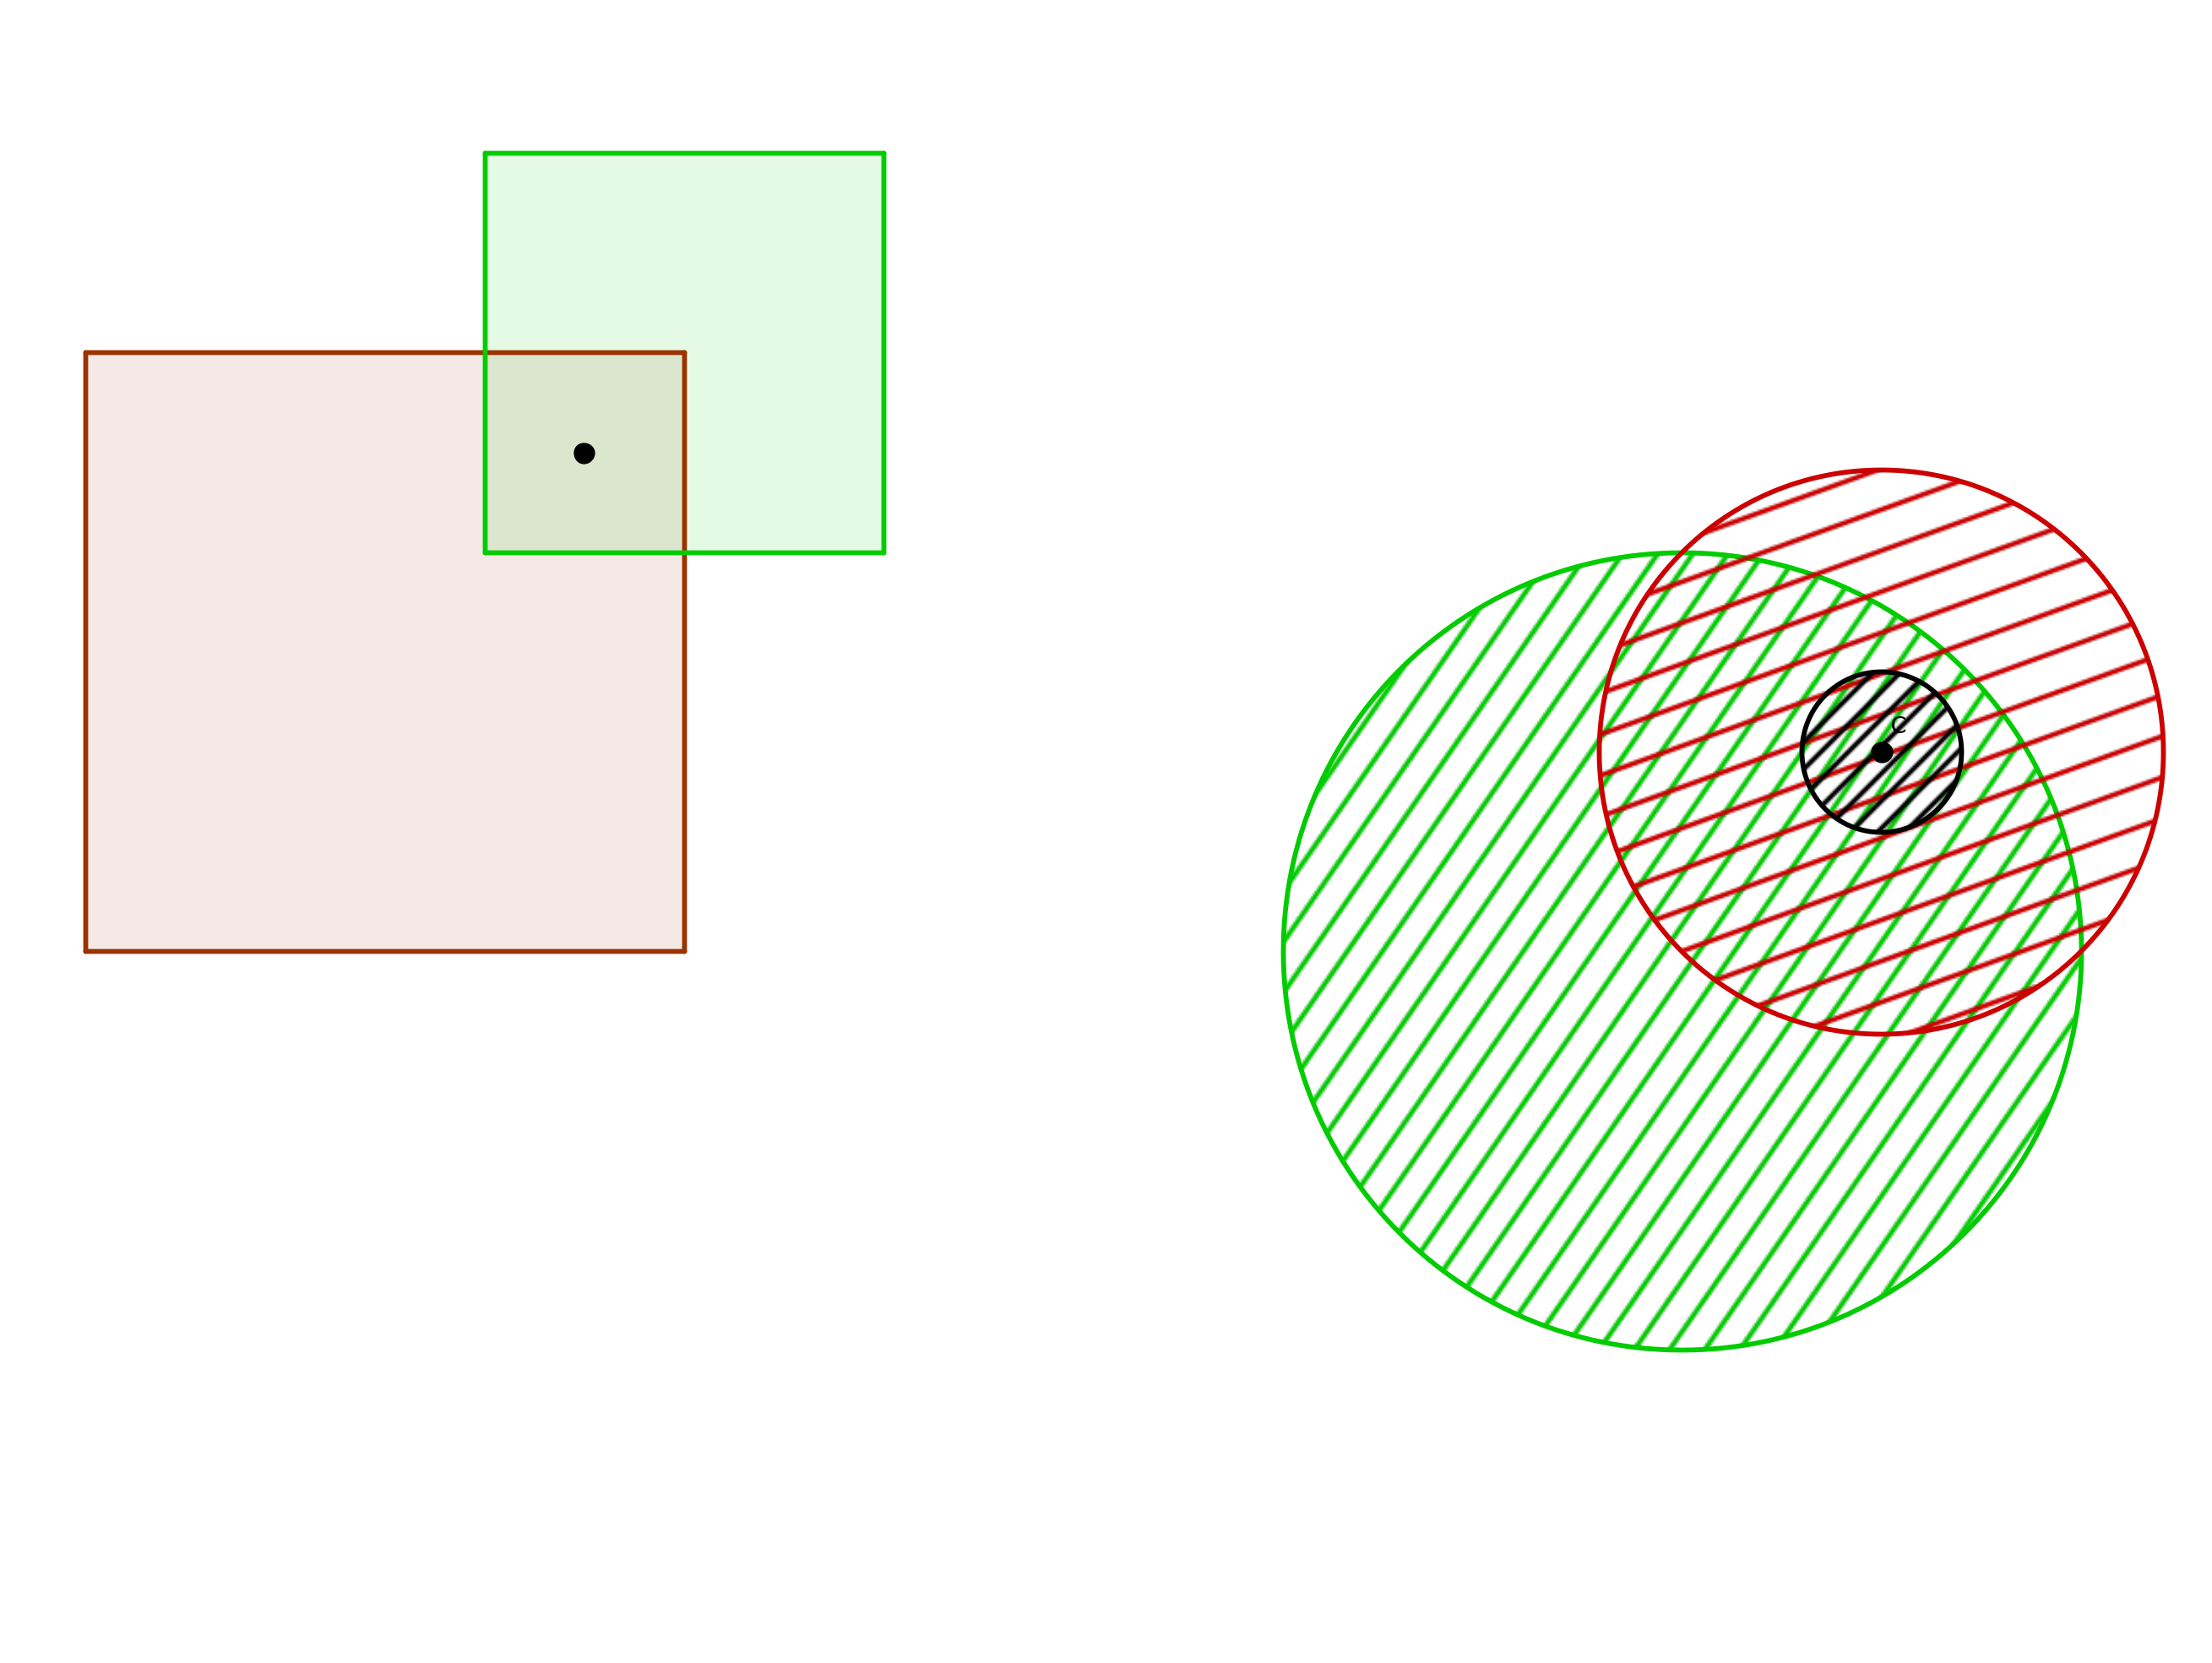
\includegraphics[scale = 0.3]{Figures/Chapter1/basesOfCircularRectangularRegions.png}
    \caption{The basis for $\Bc$ and  $\Bc'$ in  $\R \times \R$  (see example $(2)$).}
    \label{fig_1.2}
\end{figure}

\begin{lemma}\label{1.2.2}
    Let $X$ be a set, and  $\Bc$ be a basis for a topology  $\Tc$ on  $X$. Then 
    $\Tc=\{\bigcup{B}: B \in \Bc\}$.
\end{lemma}
\begin{proof}
    Given a collection $\{B\}$ of basis elements in  $\Bc$, since they are all in  $\Tc$, 
    their unions are also in $\Tc$. Conversely, given  $U \in \Tc$, then for every point 
    $x \in U$, choose a  $B_x \in \B_x$ such that  $x \in B_x \subseteq U$, then  $U=\bigcup_{x \in U}{B_x}$.
\end{proof}

%%----------------------------------------------------------------------------------------
%	SECTION 1.3
%----------------------------------------------------------------------------------------

\section{The Order Topology.}


%----------------------------------------------------------------------------------------
%	CHAPTER X
%----------------------------------------------------------------------------------------

\chapter{Sequences} % Main chapter title

\label{Chapter3} 

%----------------------------------------------------------------------------------------
%	SECTION 3.1
%----------------------------------------------------------------------------------------

\section{Some Elementary Observations} \hspace{10mm}

Consider the equation $x^2-117x+31=0$. We claim that there are no integer solutions to this equation. Let $n$ be an integer
, then $n$ is either even or odd. If $n$ is even, then so is  $n^2$ and  $17n$; hence $x^2-117x+31$ is odd. Likewise if $n$ 
is odd, then so is $n^2$ and  $117n$, thus $x^2-117x+31$ is even and so we see that $x^2-117x+31$ is never $0$.  

       				   % All the chapters goes here.
%%----------------------------------------------------------------------------------------
%	CHAPTER 4
%----------------------------------------------------------------------------------------

\chapter{Differentiability on $\R$.} % Main chapter title

\label{Chapter4} % Change X to a consecutive number; for referencing this chapter elsewhere, use \ref{ChapterX}

%% to include section files use the \input{} command.

%----------------------------------------------------------------------------------------
%	SECTION 3.1
%----------------------------------------------------------------------------------------

\section{Some Elementary Observations} \hspace{10mm}

Consider the equation $x^2-117x+31=0$. We claim that there are no integer solutions to this equation. Let $n$ be an integer
, then $n$ is either even or odd. If $n$ is even, then so is  $n^2$ and  $17n$; hence $x^2-117x+31$ is odd. Likewise if $n$ 
is odd, then so is $n^2$ and  $117n$, thus $x^2-117x+31$ is even and so we see that $x^2-117x+31$ is never $0$.  



%%----------------------------------------------------------------------------------------
%	CHAPTER X
%----------------------------------------------------------------------------------------

\chapter{Quadratic Reciprocity} % Main chapter title

\label{ChapterX} % Change X to a consecutive number; for referencing this chapter elsewhere, use \ref{ChapterX}

%% to include section files use the \input{} command.

%----------------------------------------------------------------------------------------
%	SECTION 3.1
%----------------------------------------------------------------------------------------

\section{Some Elementary Observations} \hspace{10mm}

Consider the equation $x^2-117x+31=0$. We claim that there are no integer solutions to this equation. Let $n$ be an integer
, then $n$ is either even or odd. If $n$ is even, then so is  $n^2$ and  $17n$; hence $x^2-117x+31$ is odd. Likewise if $n$ 
is odd, then so is $n^2$ and  $117n$, thus $x^2-117x+31$ is even and so we see that $x^2-117x+31$ is never $0$.  

%----------------------------------------------------------------------------------------
%	SECTION 1.2
%----------------------------------------------------------------------------------------

\section{The Basis and Subbasis for a Topology.}

\begin{definition}
    If $X$ is a set, the \textbf{basis} for a topology on $X$ is a collection $\Bc$ of 
    subsets of  $X$, called \textbf{basis elements}, such that:
        \begin{enumerate}[label=(\arabic*)]
            \item For every $x \in X$, there is a  $B \in \Bc$ such that $x \in B$.

            \item For $B_1,B_2 \in \Bc$, if $x \in B_1 \cap B_2$, then there is a $B_3 \in \Bc$ 
                such that $x \in B_3 \subseteq B_1 \cap B_2$
        \end{enumerate}
We define the topology $\Tc$ \textbf{generated} by $\Bc$ to be collection of open sets: 
$\Tc=\{U \subseteq X: x \in B \text{ for some } B \in \Bc\}$.
\end{definition}

\begin{theorem}\label{1.2.1}
    Let $X$ be a set, and  $\Bc$ a basis of  $X$, then the collection of subsets 
    of  $X$, $\Tc=\{U \subseteq X: x \in B \text{ for some } B \in \Bc\}$ is a topology on $X$.
\end{theorem}
\begin{proof}
    Let $\Bc$ be a basis for a topology in  $X$, and consider  $\Tc$ as defined 
    above. Cleary, $\emptyset \in X$ and so is  $X$.

    Now let  $\{U_{\alpha}\}$ be a subcollection of subsets of  $X$, and let  $U=\bigcup{U_{\alpha}}$. 
    Then if  $x \in U$ for some  $\alpha$, there is a  $B_{\alpha}$ such that  $x \in B_{\alpha} \subseteq U_{\alpha}$, 
    thus  $x \in B_{\alpha} \subseteq U$.

    Now let  $x \in  U_1 \cap U_2$, and choose $B_1,B_2 \in \Bc$ such that $x \in B_1 \subseteq U_1$ 
    and $x \in B_2 \subseteq U_2$. Then  by definition, there is a $B_3$ for which $x \in B_3 \subseteq B_1 \cap B_2$.
    Now suppose for arbitrary $n$, that  $U=\bigcap_{i=1}^{n}{U_i} \in \Tc$, for some finite 
    subcollection  $\{U_i\}$ of subsets of  $X$. Then by let  $B_n, B_{n+1} \in \Bc$ such that 
    $x \in B_n \subseteq U$ and  $x \in B_{n+1} \subseteq U_{n+1}$. Then by our hypothesis, there is a  $B$ 
for which  $x \in B \subseteq B_n \cap B_{n+1}$, thus  $U \cap U_{n+1}=\bigcap_{i=1}^{n+1}{U_i} \in \Tc$. 
This make $\Tc$ a topology on  $X$.
\end{proof}

\begin{example}
    \begin{enumerate}[label=(\arabic*)]
        \item Let $\Bc$ be the set of all circular regions in the plane  $\R \times \R$, then 
            $\Bc$ satisfies the conditions needed for a basis.

        \item The collection  $\Bc'$ in  $\R \times \R$ of all rectangular region also 
            forms a basis for a topology on  $\R \times \R$.

        \item For any set  $X$, the set of all  $1$-point elements of  $X$ forms a 
            basis for a topology on  $X$.
    \end{enumerate}		
\end{example}

\begin{figure}
    \centering
    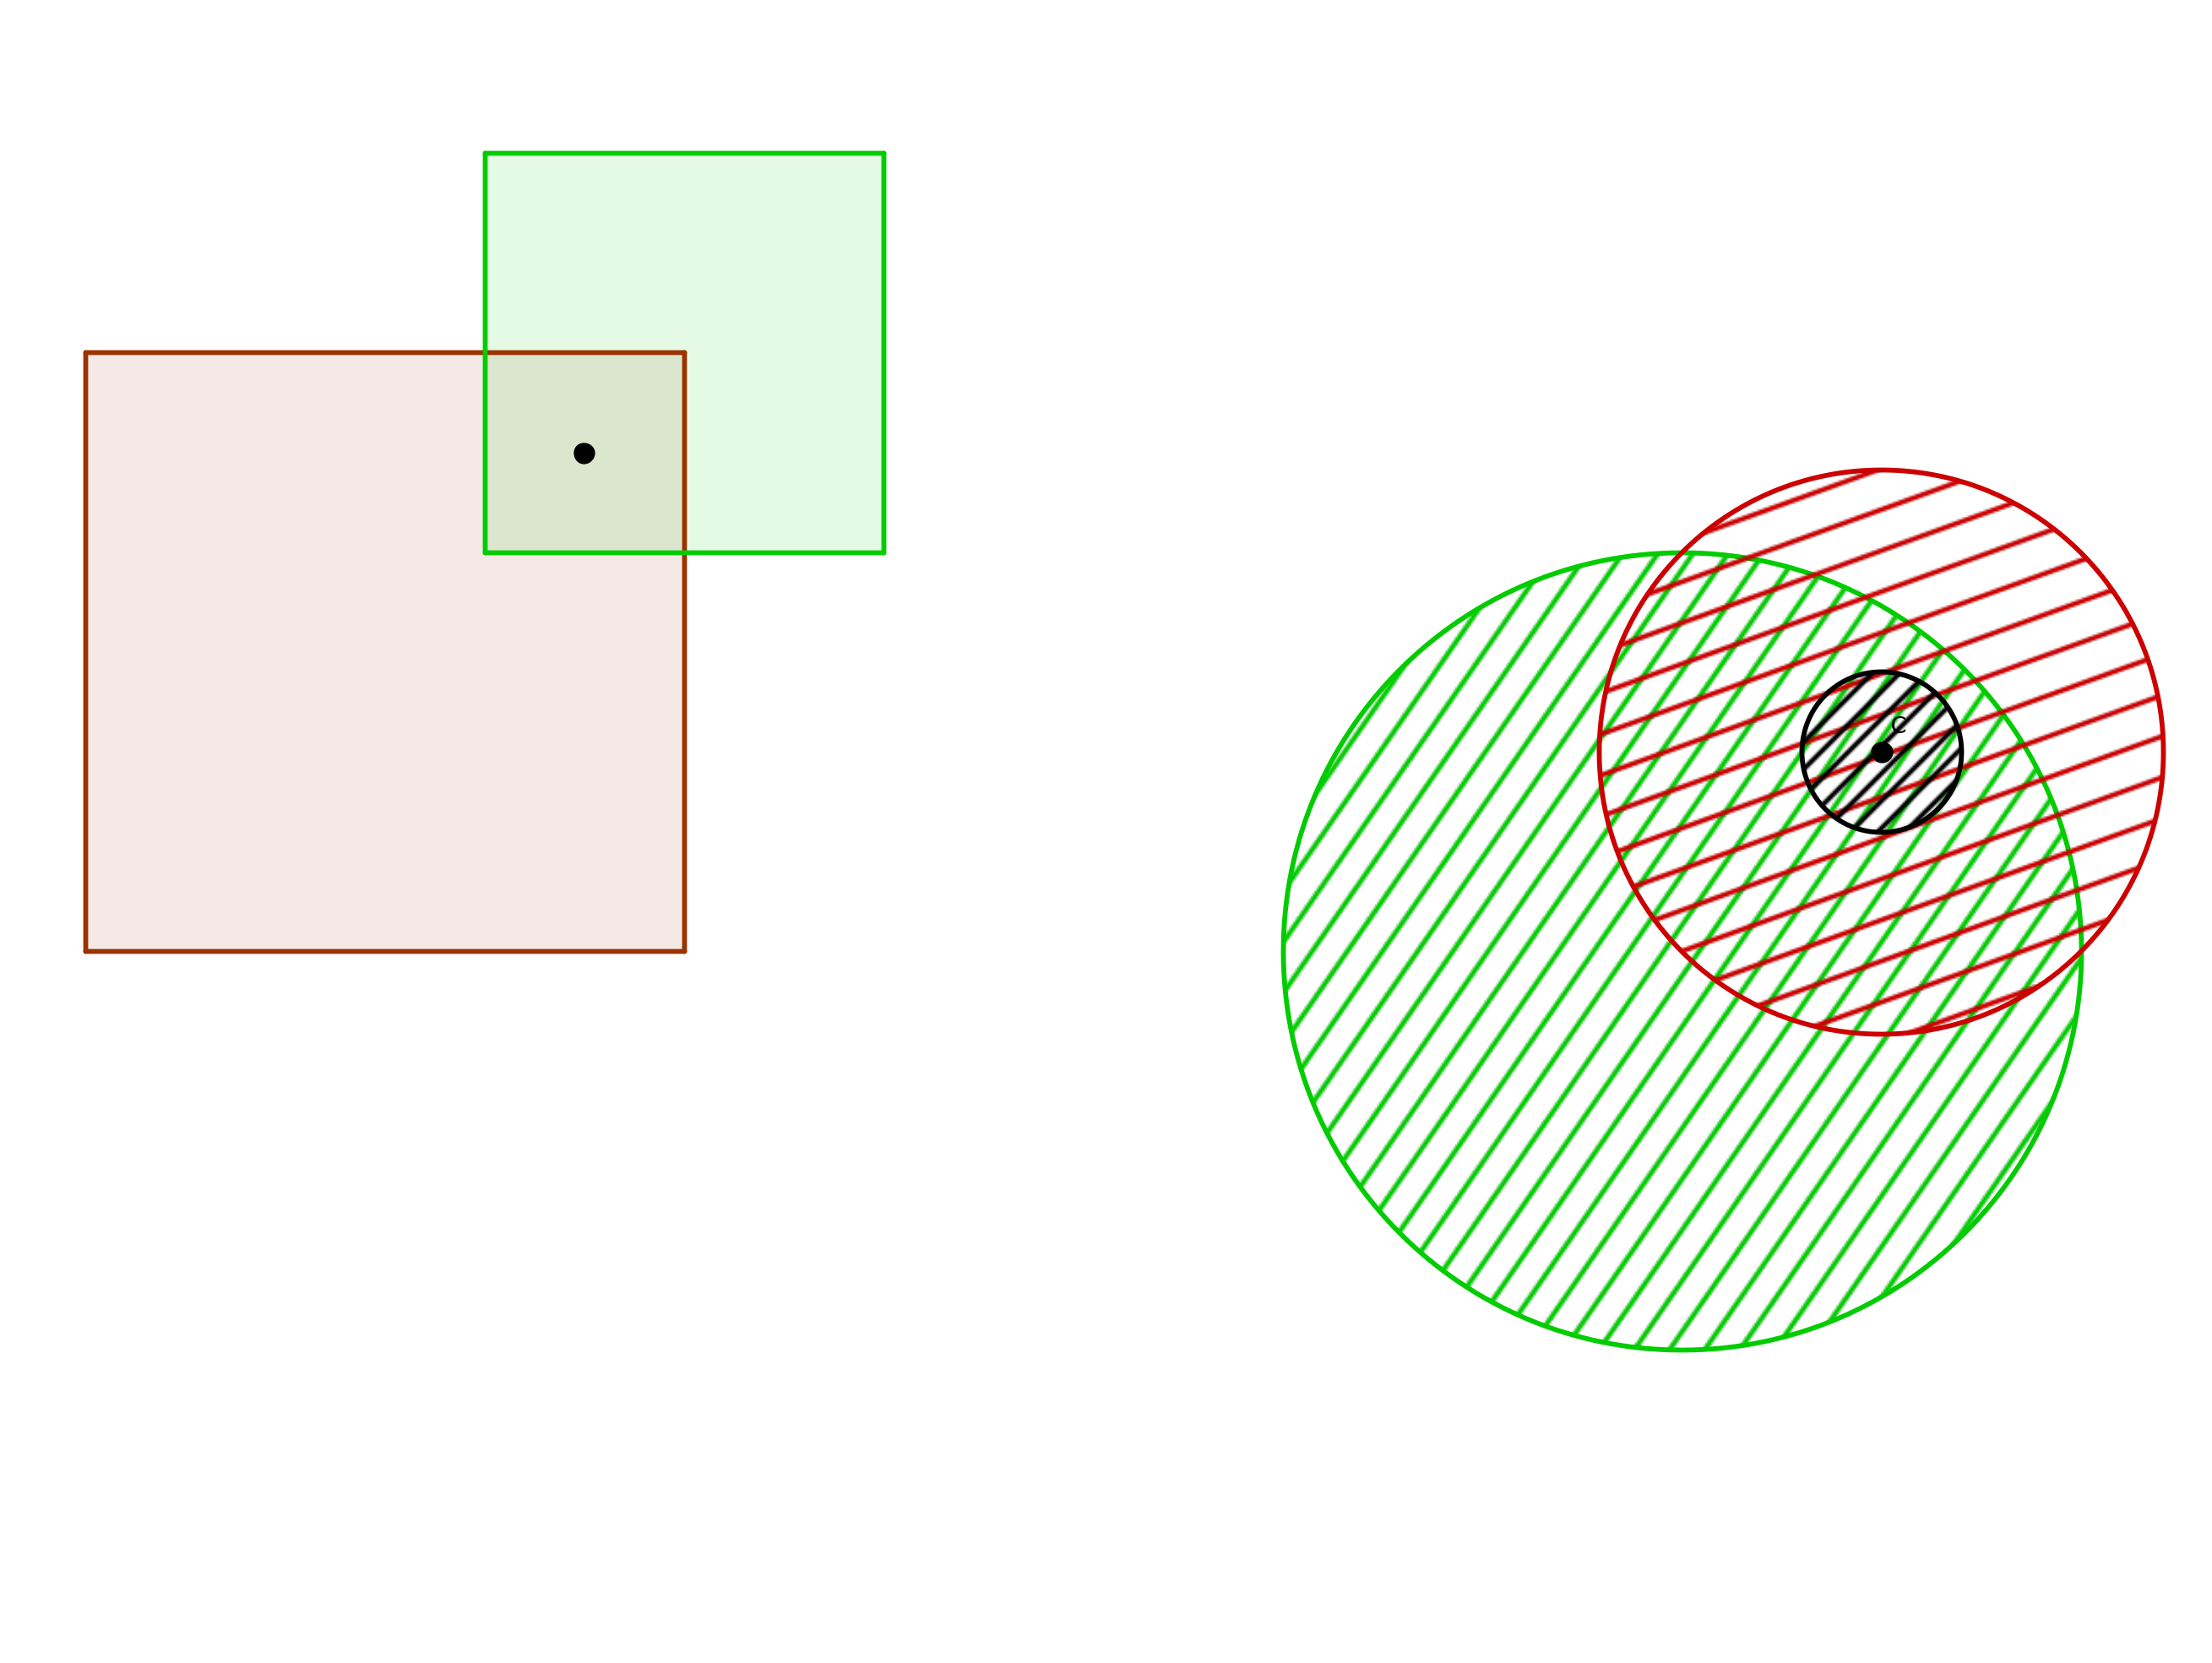
\includegraphics[scale = 0.3]{Figures/Chapter1/basesOfCircularRectangularRegions.png}
    \caption{The basis for $\Bc$ and  $\Bc'$ in  $\R \times \R$  (see example $(2)$).}
    \label{fig_1.2}
\end{figure}

\begin{lemma}\label{1.2.2}
    Let $X$ be a set, and  $\Bc$ be a basis for a topology  $\Tc$ on  $X$. Then 
    $\Tc=\{\bigcup{B}: B \in \Bc\}$.
\end{lemma}
\begin{proof}
    Given a collection $\{B\}$ of basis elements in  $\Bc$, since they are all in  $\Tc$, 
    their unions are also in $\Tc$. Conversely, given  $U \in \Tc$, then for every point 
    $x \in U$, choose a  $B_x \in \B_x$ such that  $x \in B_x \subseteq U$, then  $U=\bigcup_{x \in U}{B_x}$.
\end{proof}

%----------------------------------------------------------------------------------------
%	SECTION 1.3
%----------------------------------------------------------------------------------------

\section{The Order Topology.}

%%----------------------------------------------------------------------------------------
%	CHAPTER X
%----------------------------------------------------------------------------------------

\chapter{Differentiation} % Main chapter title

\label{Chapter6}

%----------------------------------------------------------------------------------------
%	SECTION 3.1
%----------------------------------------------------------------------------------------

\section{Some Elementary Observations} \hspace{10mm}

Consider the equation $x^2-117x+31=0$. We claim that there are no integer solutions to this equation. Let $n$ be an integer
, then $n$ is either even or odd. If $n$ is even, then so is  $n^2$ and  $17n$; hence $x^2-117x+31$ is odd. Likewise if $n$ 
is odd, then so is $n^2$ and  $117n$, thus $x^2-117x+31$ is even and so we see that $x^2-117x+31$ is never $0$.  

%----------------------------------------------------------------------------------------
%	SECTION 1.2
%----------------------------------------------------------------------------------------

\section{The Basis and Subbasis for a Topology.}

\begin{definition}
    If $X$ is a set, the \textbf{basis} for a topology on $X$ is a collection $\Bc$ of 
    subsets of  $X$, called \textbf{basis elements}, such that:
        \begin{enumerate}[label=(\arabic*)]
            \item For every $x \in X$, there is a  $B \in \Bc$ such that $x \in B$.

            \item For $B_1,B_2 \in \Bc$, if $x \in B_1 \cap B_2$, then there is a $B_3 \in \Bc$ 
                such that $x \in B_3 \subseteq B_1 \cap B_2$
        \end{enumerate}
We define the topology $\Tc$ \textbf{generated} by $\Bc$ to be collection of open sets: 
$\Tc=\{U \subseteq X: x \in B \text{ for some } B \in \Bc\}$.
\end{definition}

\begin{theorem}\label{1.2.1}
    Let $X$ be a set, and  $\Bc$ a basis of  $X$, then the collection of subsets 
    of  $X$, $\Tc=\{U \subseteq X: x \in B \text{ for some } B \in \Bc\}$ is a topology on $X$.
\end{theorem}
\begin{proof}
    Let $\Bc$ be a basis for a topology in  $X$, and consider  $\Tc$ as defined 
    above. Cleary, $\emptyset \in X$ and so is  $X$.

    Now let  $\{U_{\alpha}\}$ be a subcollection of subsets of  $X$, and let  $U=\bigcup{U_{\alpha}}$. 
    Then if  $x \in U$ for some  $\alpha$, there is a  $B_{\alpha}$ such that  $x \in B_{\alpha} \subseteq U_{\alpha}$, 
    thus  $x \in B_{\alpha} \subseteq U$.

    Now let  $x \in  U_1 \cap U_2$, and choose $B_1,B_2 \in \Bc$ such that $x \in B_1 \subseteq U_1$ 
    and $x \in B_2 \subseteq U_2$. Then  by definition, there is a $B_3$ for which $x \in B_3 \subseteq B_1 \cap B_2$.
    Now suppose for arbitrary $n$, that  $U=\bigcap_{i=1}^{n}{U_i} \in \Tc$, for some finite 
    subcollection  $\{U_i\}$ of subsets of  $X$. Then by let  $B_n, B_{n+1} \in \Bc$ such that 
    $x \in B_n \subseteq U$ and  $x \in B_{n+1} \subseteq U_{n+1}$. Then by our hypothesis, there is a  $B$ 
for which  $x \in B \subseteq B_n \cap B_{n+1}$, thus  $U \cap U_{n+1}=\bigcap_{i=1}^{n+1}{U_i} \in \Tc$. 
This make $\Tc$ a topology on  $X$.
\end{proof}

\begin{example}
    \begin{enumerate}[label=(\arabic*)]
        \item Let $\Bc$ be the set of all circular regions in the plane  $\R \times \R$, then 
            $\Bc$ satisfies the conditions needed for a basis.

        \item The collection  $\Bc'$ in  $\R \times \R$ of all rectangular region also 
            forms a basis for a topology on  $\R \times \R$.

        \item For any set  $X$, the set of all  $1$-point elements of  $X$ forms a 
            basis for a topology on  $X$.
    \end{enumerate}		
\end{example}

\begin{figure}
    \centering
    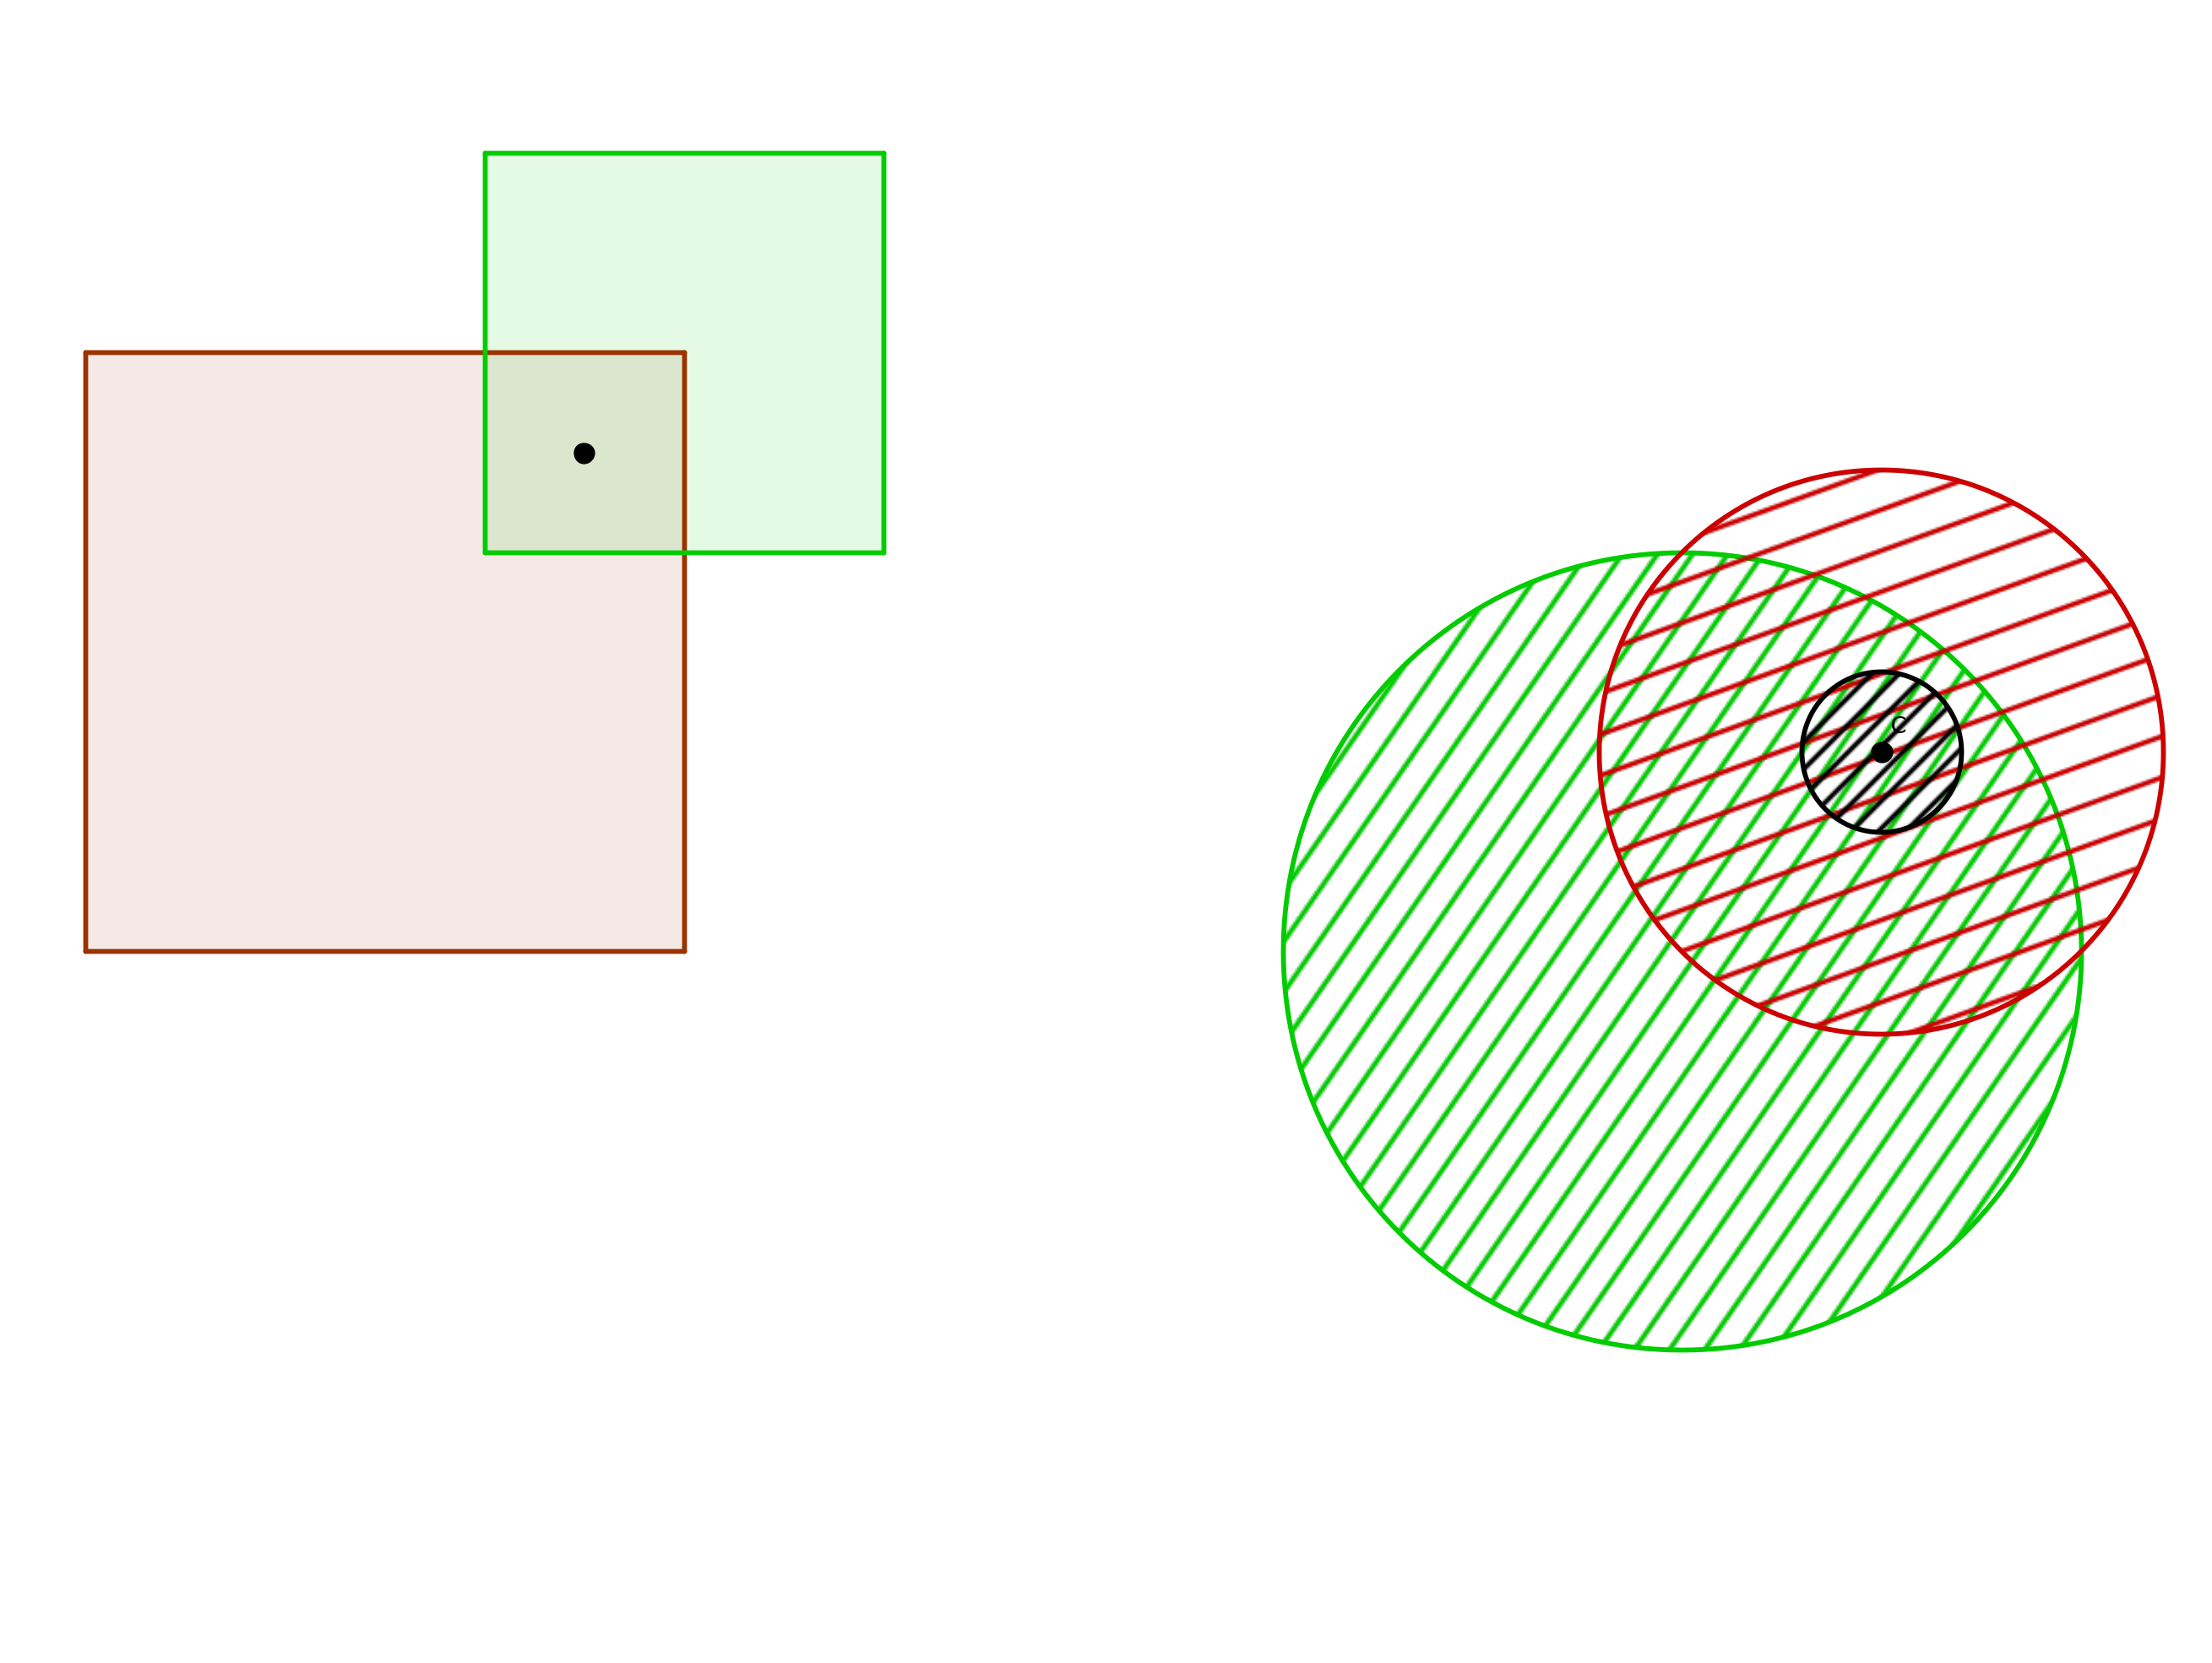
\includegraphics[scale = 0.3]{Figures/Chapter1/basesOfCircularRectangularRegions.png}
    \caption{The basis for $\Bc$ and  $\Bc'$ in  $\R \times \R$  (see example $(2)$).}
    \label{fig_1.2}
\end{figure}

\begin{lemma}\label{1.2.2}
    Let $X$ be a set, and  $\Bc$ be a basis for a topology  $\Tc$ on  $X$. Then 
    $\Tc=\{\bigcup{B}: B \in \Bc\}$.
\end{lemma}
\begin{proof}
    Given a collection $\{B\}$ of basis elements in  $\Bc$, since they are all in  $\Tc$, 
    their unions are also in $\Tc$. Conversely, given  $U \in \Tc$, then for every point 
    $x \in U$, choose a  $B_x \in \B_x$ such that  $x \in B_x \subseteq U$, then  $U=\bigcup_{x \in U}{B_x}$.
\end{proof}

%----------------------------------------------------------------------------------------
%	SECTION 1.3
%----------------------------------------------------------------------------------------

\section{The Order Topology.}

%----------------------------------------------------------------------------------------
%	SECTION 4.3
%----------------------------------------------------------------------------------------

\section{Monotonic Functions and Inverse Functions.}

\begin{definition}
    Let $E \subseteq \R$ be nonempty, and let  $f:E \rightarrow \R$ be a realvalued function. 
    We say that $f$ is \textbf{monotonically increasing} on $E$ if for $x<y$, $f(x) \leq f(y)$. 
    Similarly, $f$ is \textbf{monotonically decreasing} if $f(y) \leq f(x)$. In either case, we call 
    $f$ a \textbf{monotonic} function.
\end{definition}

\begin{example}
    The function $f(x)=x^2$ is not monotonoic on  $I$, but it is monotonically increasing 
    over $[0,\infty)$ and monotonically decreasing over $(-\infty, 0)$. 
\end{example} 

\begin{theorem}\label{4.4.1}
    Suppose that $a, b \in \R$ , with  $a$ and  $b$ distinct, and let  $f$ be contiuous 
    over  $[a,b]$ and differentiable over  $(a,b)$. Then:
        \begin{enumerate}[label=(\arabic*)]
            \item If $f' \geq 0$, for all  $x \in (a,b)$, then $f$ monotonically increasing 
                on $[a,b]$; respectively, if  $f' \leq 0$,  $f$ is monotonically decreasing.

            \item If $f'=0$, for all  $x \in (a,b)$, then $f$ is constant on  $[a,b]$
        \end{enumerate}
\end{theorem}
\begin{proof}
    Assume without loss of generality that $f' \leq 0$, then for any  $a<x_1<x_2<b$, then 
    $f$ is continuous on  $[x_1,x_2]$ and differentiable on $(x_1,x_2)$, hence by the 
    mean value theorem, then there is a $c \in (x_1,x_2)$ such that $f(x_2)f(x_1)=f'(c)(x_2-x_1)$, 
    hence $f(x_2)-f(x_1) \leq 0$, hence $f$ is monotonically decreasing. The case is analogous 
    for  $f'>0$.

    Now suppose that  $f'=0$,  then again by the mean value theorem, there is a  $c \in (x_1,x_2)$ 
    such that $f(x_2)-f(x_1)=f'(c)(x_2-x_1)$, then $f(x_2)-f(x_2)=0$, for $x_1, x_2 \in (a,b)$ 
    arbitrary therefore, $f$ is constant.
\end{proof}

\begin{remark}
    If $f$ and  $g$ are continuous on a nondegenerate inteval,  $[a,b]$, and differentiable 
    on  $(a,b)$, and  $f'=g'$ for all  $x \in (a,b)$, then $f-g$ is constant.
\end{remark}
\begin{proof}
    We repeat the proof for the constant case using the Cauchy mean value theorem; 
    similarly, we can just apply the previous theorem to the function $f-g$.
\end{proof}

Suppose that $f$ is a realvalued function, who has an inverse function  $f^{-1}$. Then 
the graph of  $f^{-1}$ is symmetric to the graph of  $f$ with respect to the line  $y=x$. Then 
visually,  $f^{-1}$ is as smooth as  $f$. Algebraically, we can apply an operation to the graph 
of $f$ to obtain the graph of  $f^{-1}$, and we can observe that smoothness is preserved, however 
we would like to prove this rigorously.

\begin{theorem}\label{4.4.2}
    If $f$ is a  1-1 continuous function of the interval  $I$ onto $\R$, 
    then  $f$ is strictly monotonic on  $I$, and  $f^{-1}$ is continuous and strictly 
    monotonic on $f(I)$.
\end{theorem}
\begin{proof}
    We have that since $f$ is 1-1, then  $f(x)=f(y)$ implies  $x=y$, hence if  $x<y$ 
    are in $I$, then  either $f(x)<f(y)$ or  $f(x)>f(y)$, now if  $f$ is not strictly monotone, then 
    for some $c \in I$, with  $x<c<y$, we have that either  $f(x)$ is inbetween $f(c)$ and  $f(b)$, 
    or  $f(y)$ is between  $f(x)$ and  $f(c)$, hence, by the intermediate value theorem, there is an  $x_1 \in I$ 
    such that $f(x_1)=f(x)$ or $f(x_1)=f(y)$. Then either $x_1=x$ or $x_2=y$ which contradicts the assumption.

    Now suppos that $f$ is strictly increasing on  $I$, since  $f$ is 1-1 ont  $\R$, then 
    $f^{-1}$ exists on  $f(I)$. Now suppose that there are  $y_1,y_2 \in f(I)$ such that 
    $ y_1<y_2$ but $f^{-1}(y_1) \geq f^{-1}(y_2)$, and since $f$ is increasing, then  $f(x_1) \geq f(x_2)$, which 
    is absurd. We also have that $f(I)$ is an interval for if  $I=[a,b]$, then  $f([a,b])=[f(a)f(b)]$ by 
    the intermediate value theorem.

    Now fix  $y_0 \in f(I)$, and let $\epsilon>0$, since $f^{-1}$ is strictly increasing, on $f(I)$ by 
    the above assumption, if $y_0$ is not a right endpoint of $f(I)$, then  $f^{-1}(y_0)$ is not 
    a  right endpoint of  $I$, then  there is an $0<\epsilon_0<\epsilon$ with $\epsilon+\epsilon_0 \in I$. Let  $\delta=f(x_0+\epsilon_0)-f(x_0)$, 
    and suppose that $0<y-y_0<\delta$, then $y_0<y<y_0+\delta=f(x_0+\epsilon_0)$, then since $f^{-1}$ is strictly 
    increasing, it follows that  $x_0<x<x+\epsilon_0$, hence we have that $0<f^{-1}(y)-f^{-1}(y_0)<\epsilon$, 
    that is $f^{-1}(y_0+)$ exists, similatly, if $y_0$ is not a left endpoint of $I$, then  $f^{-1}(y_0-)$ 
    exists. In both cases, we have that $f^{-1}(y_0\pm)=f(y_0)$. Therefore, $f^{-1}$ is contiuous.
\end{proof}

\begin{theorem}[The Inverse Function Theorem]\label{4.4.3}
    Let $f$ be a 1-1 continuous function of an open interval  $I$ onto  $\R$. If  $a \in f(I)$, 
    and if  $f'(f^{-1}(a)) \neq 0$ exists, then  $f^{-1}$ is differentiable at $a$, and 
        \begin{equation}
            (f^{-1})'=\frac{1}{f'}
        \end{equation} 
\end{theorem}
\begin{proof}
    We have that $f(f(^{-1})(x))=x$, if $f$ and $f^{-1}$ are both differentiable, then 
    the chain rule yields the appropriate result. It remains to show that  $f^{-1}$ is 
    differentiable.

    By the previous theorem, we have that  $f$ is strictly monotonic, and say, without 
    loss of generalilty, that  $f$ is strictly increasing. Then  $f^{-1}$ exists, is continuous, and 
    is strictly increasing on $f(I)$. Let  $x_0=f^{-1}(a)$, then there are $c,d \in I$ such that 
    $x_0 \in (c,d) \subseteq I$, thus by the intermediate value theorem, we have that  $f((c,d))=(f(c),f(d))$ which 
    contains  $f(x_0)=a$. Then for $h \neq 0$ sufficiently small  $a+h \in (f(c),f(d))$, 
    hence $f^{-1}(a+h)$ is well defined. Now let  $x=f^{-1}(a+h)$, then  $f(x)=a+h=f(x_0)+h$, 
    thus $h=f(x)-f(x_0)$. Since $f$ is continuous, we have that as  $x \rightarrow x_0$, $h \rightarrow 0$, 
    hence  $x-x_0=f^{-1}(a+h)-f^{-1}(a) \rightarrow 0$, hence $\frac{f^{-1}(a+h)-f^{-1}(a)}{h}=
    \frac{x-x_0}{f(x)-f(x_0)}$ which exists by the continuity of $f$, thus  $f^{-1}$ is differentiable at  $a$.
\end{proof}

\begin{example}
    Take $f(x)=1$ for  $x \in \Q$ and  $f(x)=0$ for  $x \in \com{\R}{\Q}$, which is not 
    continuous at any $x$, also notice that  $x$ is not monotonic.
\end{example}

\begin{lemma}\label{4.4.4}
    Suppose that $f$ is monotonic on  $[a,b]$, if  $x_0 \in [a,b)$, then $f(x_0+)$ exists and 
    $f(x_0) \leq f(x_0+)$ or $f(x_0) \geq f(x_0+)$ (if it is increasing or decreasing respectively). Moreover, 
    if $x_0 \in (a,b]$, then $f(x_0-)$ exists and $f(x_0-) \leq f(x_0)$ or $f(x_0-) \geq f(x_0)$.
\end{lemma}
\begin{proof}
    Fix $x_0 \in [a,b]$, by the symmetry, it suffices to show that $f(x_0-)$ exists and that 
    $f(x_0-) \leq f(x_0)$ if $f$ is increasing. Set  $E=\{f(x):a<x<x_0\}$ and let $s=\sup{E}$. We have 
    $f (x_0)$ is an upeprbound, thus $s$ is finite, and  $s \leq f(x_0)$. It remains to show that $s=f(x_0-)$.

    Now given $\epsilon>0$, by the approximation property, there is an $x_1 \in (a,x_0)$ such that 
    $s-\epsilon<f(x) \leq s$. Since  $f$ is increasing, then we have  $s-\epsilon<f(x_1)<f(x) \leq s$, so 
    choose $\delta=x_0-x_1>0$, then for $-\delta<x-x_0<0$, we have that $|f(x)-s|<\epsilon$, and we are 
    done.
\end{proof}

\begin{theorem}\label{4.4.5}
    If $f$ is monotonic on an interval  $I$, then  $f$ has at most countably many discontinuities on  $I$.
\end{theorem}
\begin{proof}
    Suppose that $f$ is monotonically increasing, without loss of generality. We know that the 
    countable union of atmost countable sets is countable. It suffices to show that the set 
    of all discontinuities of  $f$ is a coutnable union of atmost countable sets.

    Notice that  $\R=\bigcup_{n=1}^{\infty}{[-n,n]}$, now let  $I$ be a closed, bounded, interval  $[a,b]$, 
    and let $E$ be the set of all discontinuities of  $f$ on  $(a,b)$. By lemma \ref{4.4.4}, we have that 
    $f(x-) \leq f(x) \leq f(x+)$, then we see that  $f$ is discontinuous at  $x$ if and only if  $0<f(x+)-f(x-)$. 
    Let  $A_j=\{x \in I: f(x+)-f(x-) \geq \frac{1}{j}\}$, then $A_j \subseteq E$, and we have 
    $E=\bigcup_{j=1}^{\infty}{A_j}$. We would like to show that  $A_j$ is finite for all  $j$.

    For suppose not, then there is a  $j_0$ such that $A_{j_0}$ is infinite, then pick $a \leq x_1<x_2<\dots 
    \leq b\in A_{j_0}$, with $f(x_k+)-f(x_k-)>\frac{1}{j_0}$ for all $k$. Then $f(b)-f(a) \geq f(b)-f(x_1-) 
    \geq f(x_1+)-f(x_1-)>\frac{1}{j_0} \geq f(x_2+)-f(x_1-)=f(x_2+)-f(x_2-)+f(x_2-)-f(x_1-)>\frac{1}{j_0}$, 
    continuing along this line, we get that $f(b)-f(a) \geq \frac{n}{j_0}$ for all $n \geq 1$, which 
    implies that  $f(b)-f(a)$ is infinite, which is a contradiction. Thus  $A_j$ must be finite.
\end{proof}

\begin{figure}
    \centering
    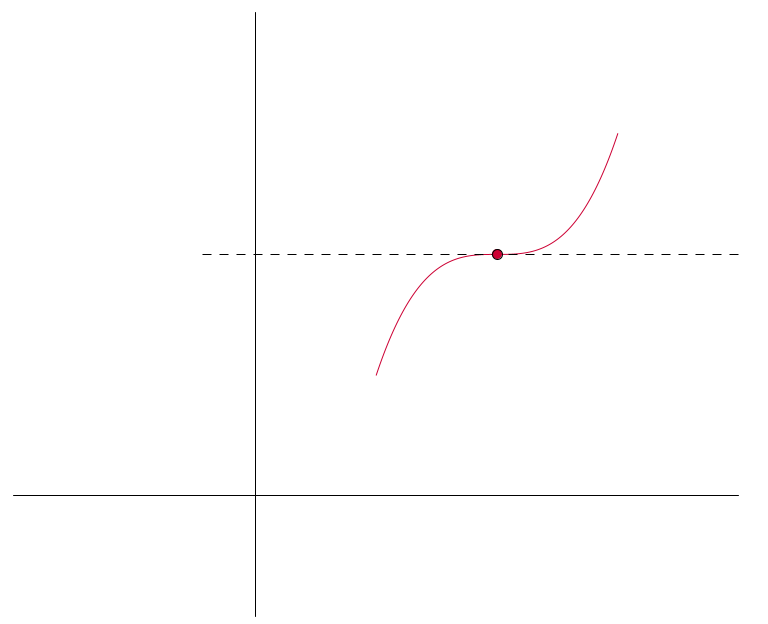
\includegraphics[scale = 0.3]{figures/meanValueDeriv.png}
    \caption{The intermediate value theorem for derviavtives.}
    \label{fig_4.2}
\end{figure}

\begin{theorem}[The Intermediate Value Theorem for Derivatives]\label{4.4.5}
    Suppose that $f$ is differentiable on a closed interval  $[a,b]$, where  $f'(a) \neq g('b)$. If  $y_0 \in \R$ such that $f'(a)<y_0<f'(b)$, then there is an $x_0 \in (a,b)$ such that $f'(x_0)=y_0$.
\end{theorem}
\begin{proof}
    Suppose that $f'(a)<y_0<f'(b)$, now suppose without loss of generality that $f'(a)<f'(b)$. Now let $F(x)=f(x)-y_0x$, for $x \in [a,b]$. We have that $F$ is differentiable on  $(a,b)$, then by the extreme value theorem, $F$ has a local maximum, and a local minumum, let  $F(x_0)$ is a local minimum on $[a,b]$. We have that  $F'(a)=f'(a)-y_0<0$, which is decreasing, so for $h$ sufficiently small, we have  $F(a+h)-F(a)<0$, hence  $F(a)$ cannot be the minumum, hence  $x_0 \neq a$. Similarly,
    $F'(b)=f'(b)-y_0>0$, which is increasing, by similar reasoning, we have that $F(b+h)-F(b)>0$ for  $h$ sufficiently small, hence $F(b)$ cannot be a local maximum, so  $x_0 \neq b$. Thus $x_0 \in (a,b)$. Now since $F(x_0)$ is a local minumum, then we have that $F'(x_0)=0$, hence $f'(x_0)=y_0$
\end{proof}
\begin{remark}
    If in the proof we assume that $f'(a)>y_0>f'(b)$, then we consider $F(x_0)$ to be a local maximum.
\end{remark}

%----------------------------------------------------------------------------------------
%	SECTION 1.1
%----------------------------------------------------------------------------------------

\section{Special Sequences}

\begin{theorem}\label{3.5.1}
    Let $n, p \in \Z^+$. Then the following hold as  $n \rightarrow \infty$.
        \begin{enumerate}[label=(\arabic*)]
            \item $\lim{\frac{1}{n^p}}=0$.

            \item $\lim{\sqrt[p]{n}}=1$.

            \item $\lim{\sqrt[n]{n}}=1$.

            \item If $\alpha \in \R$, then  $\lim{\frac{n^{\alpha}}{(1+p)^n}}=0$.

            \item If $|x|<1$, then  $\lim{x^n}=0$.
        \end{enumerate}
\end{theorem}
\begin{proof}
   \begin{enumerate}[label=(\arabic*)]
       \item Let $n>\sqry[p]{\frac{1}{\epsilon}}$; then $|\frac{1}{n^p}|<\epsilon$.

       \item If $p=1$, we are done. If  $p>1$, let  $x_n=\sqrt[n]{p}-1$, then  $x_n>0$. 
           By the binomial theorem, $1+nx_n \leq (1+x_n)^p=p$, hence $0 \leq x_n \leq \frac{p-1}{p}$. 
           Now if $1>p>0$, then  $ \frac{1}{p}>0$, so we notice that $0 \leq \frac{1}{x_n} \leq \frac{1}{\frac{p-1}{n}}$.

       \item Let $x_n=\sqrt[n]{n}-1$, then  $x_n \geq 0$, then by the binomial theorem again, 
           $n=(1+x_n)^n \geq \frac{n(n-1)}{2}x_n^2$, then $0 \leq x_n \leq \sqrt{\frac{2}{n-1}}$.

       \item Let $k \in \Z^+$ such that  $k>\alpha$. Then  $n>2k$,let  $(1+p)^n> {n \choose k}p^k>
           \frac{n^kp^k}{2^kk!}$. So $0<\frac{n^{\alpha}}{(1+p)^n}<\frac{2^kk!}{p^k}n^{\alha-k}$, since 
           $\alpha-k<0$,  $n^{\alpha-k} \rightarrow 0$ and we are done.

       \item Take  $\alpha=0$, and let  $x=\frac{1}{1+p}$, then the result follow.
   \end{enumerate} 		
\end{proof}

%----------------------------------------------------------------------------------------
%	SECTION 1.1
%----------------------------------------------------------------------------------------

\section{Monotonic Functions.}

\begin{definition}
    Let $f$ be a realvalued function on an interval  $(a,b)$. We say that  $f$ is 
    \textbf{monotonically increasing} on $(a,b)$ if  $a<x<y<b$ implies  $f(x) \leq f(y)$. 
    We say that  $f$ is \textbf{monotonically decreasing} on $(a,b)$ if  $a<x<y<b$ 
    implies  $f(y) \leq f(x)$. We say $f$ is \textbf{monotonic} if it is either monotonically 
    increasing or monotonically decreasing.
\end{definition}

\begin{theorem}\label{5.6.1}
    Let $f$ be monotonic on $(a,b)$ then $f(x+)$ and  $f(x-)$ exist at every point of 
    $(a,b)$ and $\sup{f}=f(x-)$ and  $\inf{f}=f(x+)$, and the following hold:
        \begin{enumerate}[label=(\arabic*)]
            \begin{enumerate}[label=(\arabic*)]
                \item If $f$ is monotonically increasing $f(x-) \leq f(x) \leq f(x+)$

                \item If $f$ is monotonically decreasing $f(x+) \leq f(x) \leq f(x-)$
            \end{enumerate}		
        \end{enumerate}
\end{theorem}
\begin{proof}
    We prove only $(1)$, since  $(2)$ is analogous. Suppose that $f$ is monotonically 
    increasing, clearly,  $f$ has an upperbound  $A$ for which  $A \leq f$. Now let  $\epsilon>0$, 
    then there is a  $\delta>0$ for which  $a<x-\delta<x$, and  $A-\epsilon<f(x-\delta) \leq A$.  Then we have 
    $f(x-\delta)<f(t) \leq A$ for all  $x-\delta<t<x$, then we get  $|f(t)-A|<\epsilon$, hence 
    $f(x-)=A$, Similarly, we get  $f(+)-\inf{f}$. Now since  $\sup{f} \leq f \leq inf{f}$, 
    we get the desired result.
\end{proof}

\begin{corollary}
    Monotonic functions have no infinite discontinuities.		
\end{corollary}

\begin{theorem}\label{5.6.2}
    Let $f$ be monotonic on  $(a,b)$, then the set of all  points of $(a,b)$ for which 
    $f$ is  discontinuous is atmost countable.
\end{theorem}
\begin{proof}
    Suppose, without loss of generality that $g$ is monotonically increasing, and let  $E$ 
    be the set of all points of  $(a,b)$ for which  $f$ is discontinuous. By the density of 
    $\Q$ in  $\R$, for each $x \in E$ associate $r(x) \in \Q$ such that $f(x+)<f(x)<f(x-)$. 
    Since  $x_1 < x_2$ implies $f(x_1+) \leq f(x_2-)$, then $r(x_1) \neq r(x_2)$, thus 
    $x_1 \neq x_2$, and so $r$ is a 1-1 mapping of  $E$ into  $\Q$.
\end{proof}

Now, given a countable $E$ in an interval  $(a,b)$, we can construct a monotonic function $f$ that 
is discontinuous at every point in  $E$ and continuous everywhere else. Arrange  the points of  
$E$ into a sequence  $\{x_n\}$ and let  $\{c_n\}$ be a sequence such that  $c_n>0$ for 
all  $n \in \Z^+$, such that  $\sum{c_n}$ converges. Define  $f(x)=\sum_{x_n<x}{c_n}$, for 
$x \in (a,b)$. Then we have that 
    \begin{enumerate}[label=(\arabic*)]
        \item $f$ is monotonically increasing on $(a,b)$.
            
        \item $f$ is discontinuous at every point in $E$ with $f(x_n+)-f(x_n-)=c_n$.

        \item $f$ is continuous at every point in $\com{(a,b)}{E}$.
    \end{enumerate}

\begin{definition}
    Let $f$ be a realvalued function defined on an interval $(a,b)$. We say that $f$ is 
    \textbf{continuous form the right} if $f(x+)=f(x)$, and we say $f$ is \textbf{continuous from the 
    left} if $f(x-)=f(x)$.
\end{definition}


%%----------------------------------------------------------------------------------------
%	CHAPTER X
%----------------------------------------------------------------------------------------

\chapter{Finite Fields} % Main chapter title

\label{ChapterX} % Change X to a consecutive number; for referencing this chapter elsewhere, use \ref{ChapterX}

%% to include section files use the \input{} command.

%----------------------------------------------------------------------------------------
%	SECTION 3.1
%----------------------------------------------------------------------------------------

\section{Some Elementary Observations} \hspace{10mm}

Consider the equation $x^2-117x+31=0$. We claim that there are no integer solutions to this equation. Let $n$ be an integer
, then $n$ is either even or odd. If $n$ is even, then so is  $n^2$ and  $17n$; hence $x^2-117x+31$ is odd. Likewise if $n$ 
is odd, then so is $n^2$ and  $117n$, thus $x^2-117x+31$ is even and so we see that $x^2-117x+31$ is never $0$.  

%----------------------------------------------------------------------------------------
%	SECTION 1.2
%----------------------------------------------------------------------------------------

\section{The Basis and Subbasis for a Topology.}

\begin{definition}
    If $X$ is a set, the \textbf{basis} for a topology on $X$ is a collection $\Bc$ of 
    subsets of  $X$, called \textbf{basis elements}, such that:
        \begin{enumerate}[label=(\arabic*)]
            \item For every $x \in X$, there is a  $B \in \Bc$ such that $x \in B$.

            \item For $B_1,B_2 \in \Bc$, if $x \in B_1 \cap B_2$, then there is a $B_3 \in \Bc$ 
                such that $x \in B_3 \subseteq B_1 \cap B_2$
        \end{enumerate}
We define the topology $\Tc$ \textbf{generated} by $\Bc$ to be collection of open sets: 
$\Tc=\{U \subseteq X: x \in B \text{ for some } B \in \Bc\}$.
\end{definition}

\begin{theorem}\label{1.2.1}
    Let $X$ be a set, and  $\Bc$ a basis of  $X$, then the collection of subsets 
    of  $X$, $\Tc=\{U \subseteq X: x \in B \text{ for some } B \in \Bc\}$ is a topology on $X$.
\end{theorem}
\begin{proof}
    Let $\Bc$ be a basis for a topology in  $X$, and consider  $\Tc$ as defined 
    above. Cleary, $\emptyset \in X$ and so is  $X$.

    Now let  $\{U_{\alpha}\}$ be a subcollection of subsets of  $X$, and let  $U=\bigcup{U_{\alpha}}$. 
    Then if  $x \in U$ for some  $\alpha$, there is a  $B_{\alpha}$ such that  $x \in B_{\alpha} \subseteq U_{\alpha}$, 
    thus  $x \in B_{\alpha} \subseteq U$.

    Now let  $x \in  U_1 \cap U_2$, and choose $B_1,B_2 \in \Bc$ such that $x \in B_1 \subseteq U_1$ 
    and $x \in B_2 \subseteq U_2$. Then  by definition, there is a $B_3$ for which $x \in B_3 \subseteq B_1 \cap B_2$.
    Now suppose for arbitrary $n$, that  $U=\bigcap_{i=1}^{n}{U_i} \in \Tc$, for some finite 
    subcollection  $\{U_i\}$ of subsets of  $X$. Then by let  $B_n, B_{n+1} \in \Bc$ such that 
    $x \in B_n \subseteq U$ and  $x \in B_{n+1} \subseteq U_{n+1}$. Then by our hypothesis, there is a  $B$ 
for which  $x \in B \subseteq B_n \cap B_{n+1}$, thus  $U \cap U_{n+1}=\bigcap_{i=1}^{n+1}{U_i} \in \Tc$. 
This make $\Tc$ a topology on  $X$.
\end{proof}

\begin{example}
    \begin{enumerate}[label=(\arabic*)]
        \item Let $\Bc$ be the set of all circular regions in the plane  $\R \times \R$, then 
            $\Bc$ satisfies the conditions needed for a basis.

        \item The collection  $\Bc'$ in  $\R \times \R$ of all rectangular region also 
            forms a basis for a topology on  $\R \times \R$.

        \item For any set  $X$, the set of all  $1$-point elements of  $X$ forms a 
            basis for a topology on  $X$.
    \end{enumerate}		
\end{example}

\begin{figure}
    \centering
    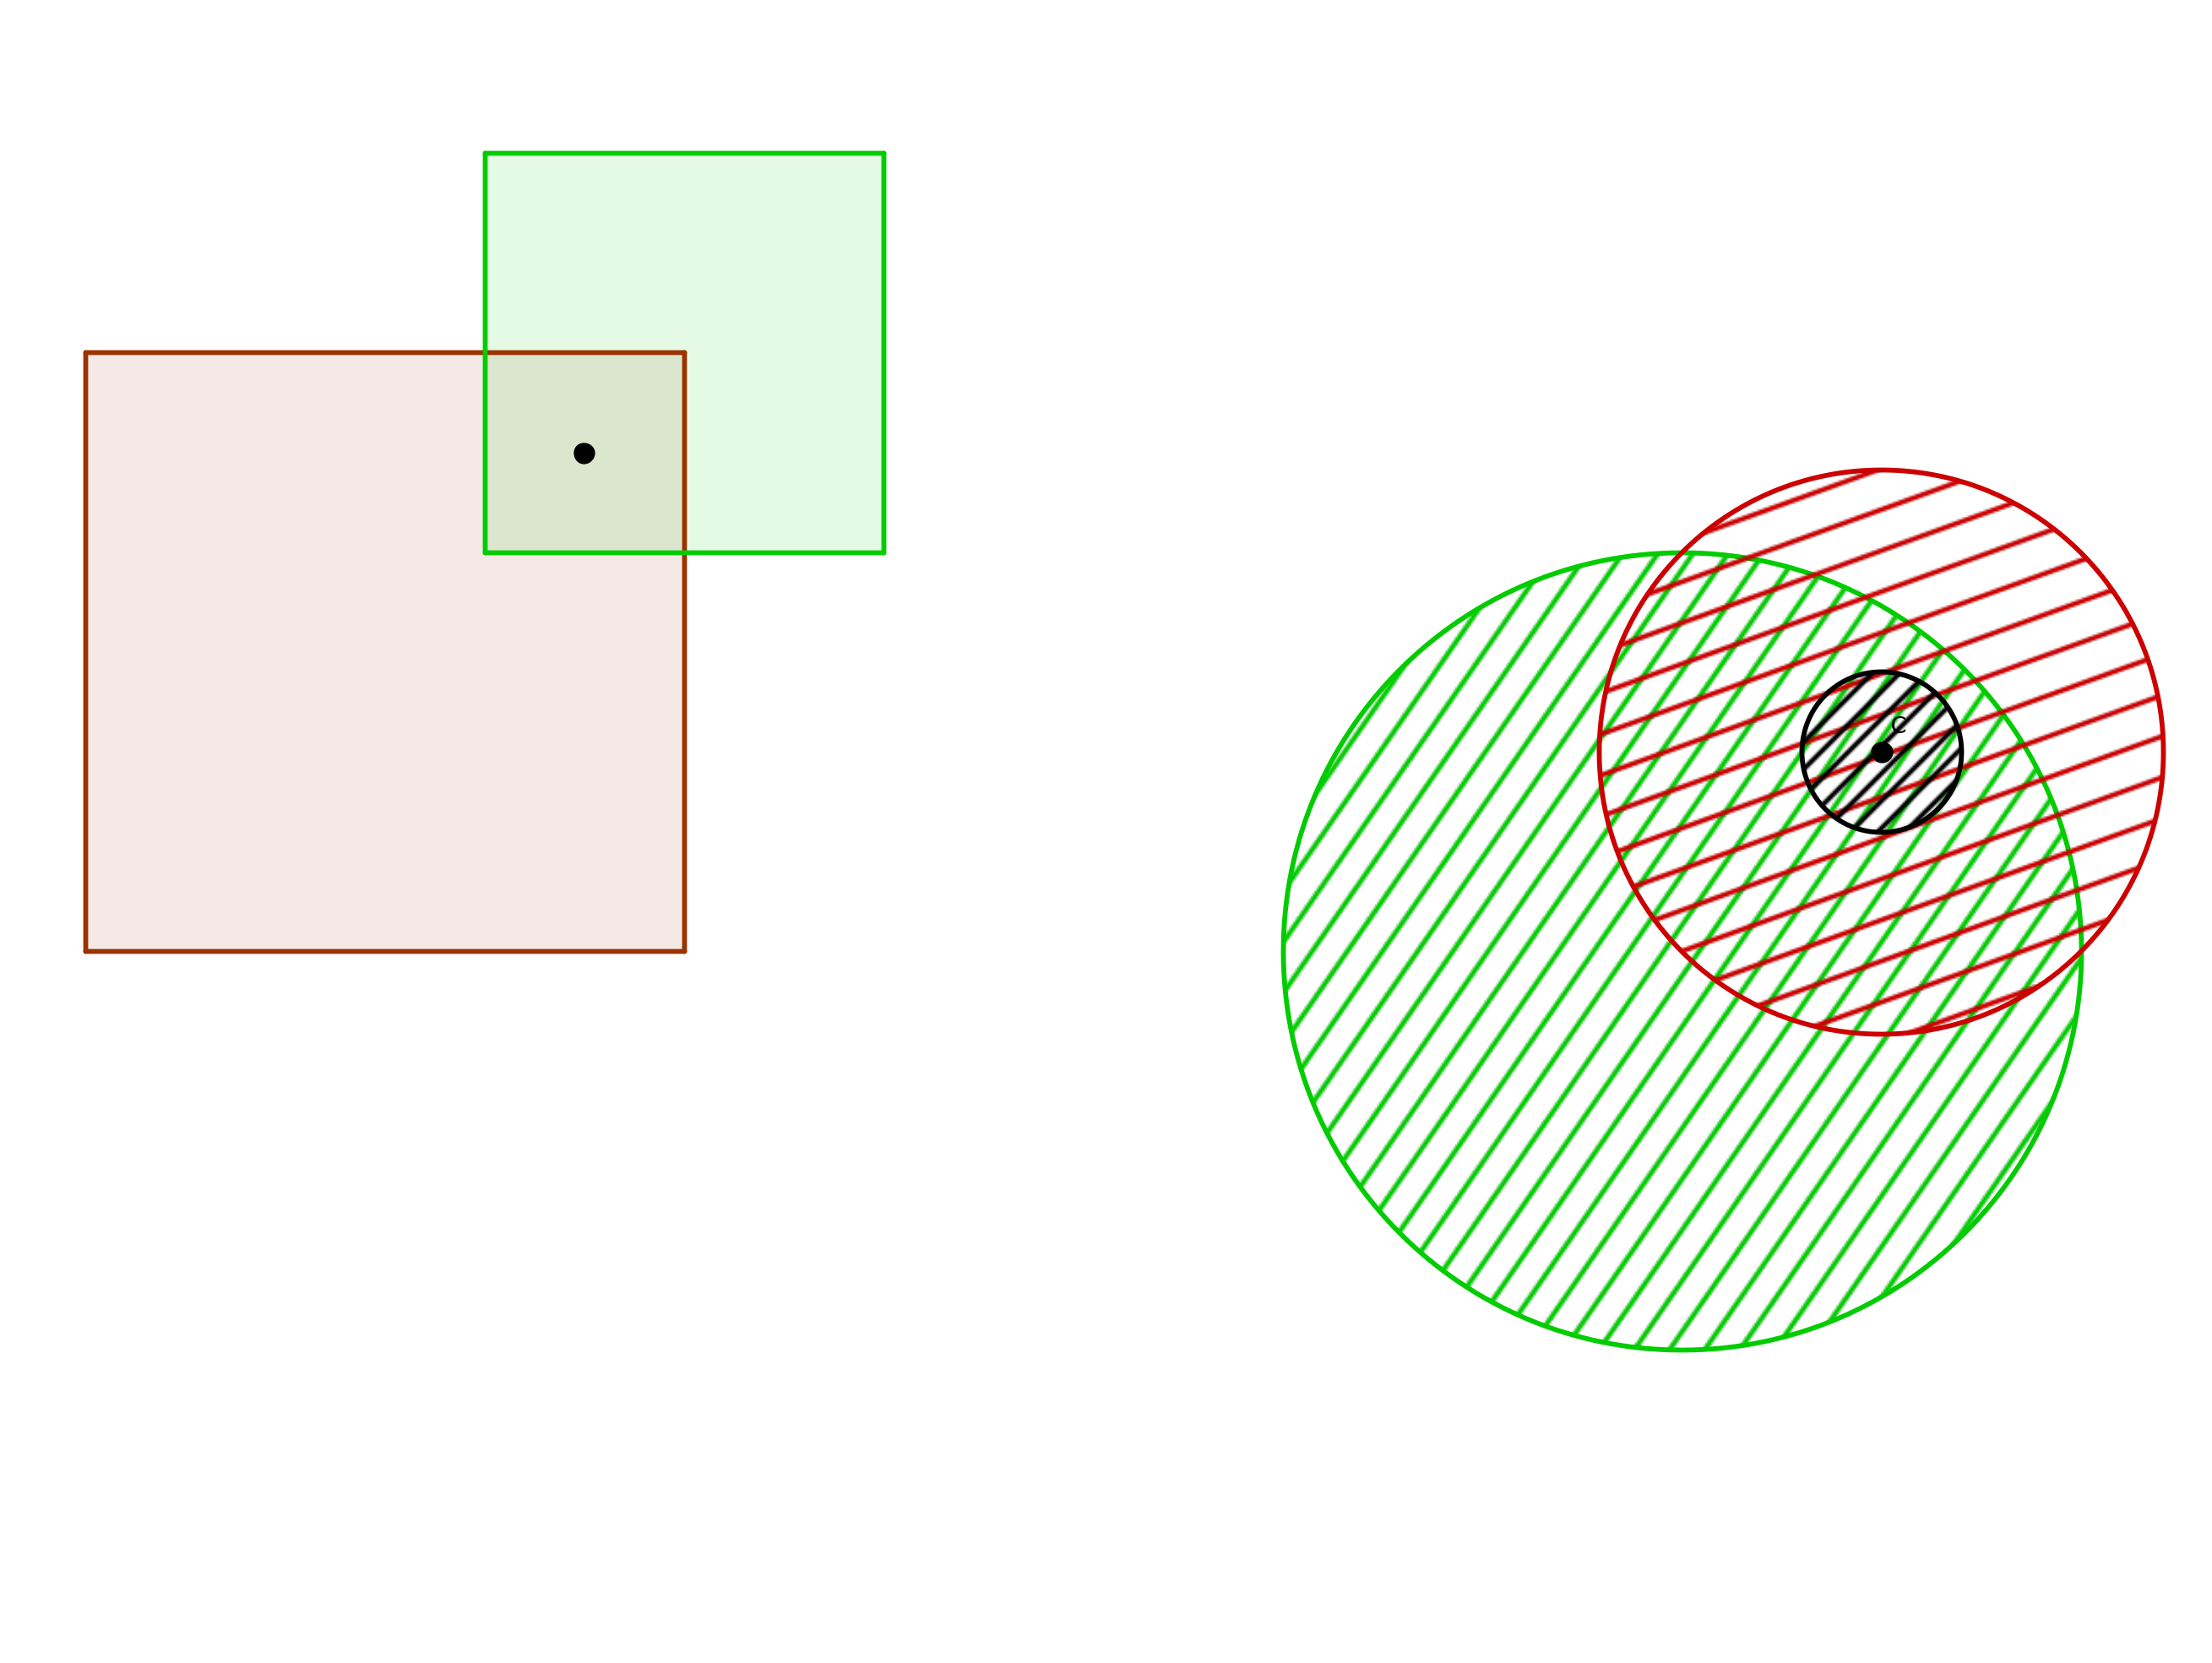
\includegraphics[scale = 0.3]{Figures/Chapter1/basesOfCircularRectangularRegions.png}
    \caption{The basis for $\Bc$ and  $\Bc'$ in  $\R \times \R$  (see example $(2)$).}
    \label{fig_1.2}
\end{figure}

\begin{lemma}\label{1.2.2}
    Let $X$ be a set, and  $\Bc$ be a basis for a topology  $\Tc$ on  $X$. Then 
    $\Tc=\{\bigcup{B}: B \in \Bc\}$.
\end{lemma}
\begin{proof}
    Given a collection $\{B\}$ of basis elements in  $\Bc$, since they are all in  $\Tc$, 
    their unions are also in $\Tc$. Conversely, given  $U \in \Tc$, then for every point 
    $x \in U$, choose a  $B_x \in \B_x$ such that  $x \in B_x \subseteq U$, then  $U=\bigcup_{x \in U}{B_x}$.
\end{proof}

%----------------------------------------------------------------------------------------
%	SECTION 1.3
%----------------------------------------------------------------------------------------

\section{The Order Topology.}

%\input{chapters/capitulo5.tex}					   % If you want add this chapter remove the comment (%).
%%----------------------------------------------------------------------------------------
%	CHAPTER X
%----------------------------------------------------------------------------------------

\chapter{Differentiation} % Main chapter title

\label{Chapter6}

%----------------------------------------------------------------------------------------
%	SECTION 3.1
%----------------------------------------------------------------------------------------

\section{Some Elementary Observations} \hspace{10mm}

Consider the equation $x^2-117x+31=0$. We claim that there are no integer solutions to this equation. Let $n$ be an integer
, then $n$ is either even or odd. If $n$ is even, then so is  $n^2$ and  $17n$; hence $x^2-117x+31$ is odd. Likewise if $n$ 
is odd, then so is $n^2$ and  $117n$, thus $x^2-117x+31$ is even and so we see that $x^2-117x+31$ is never $0$.  

%----------------------------------------------------------------------------------------
%	SECTION 1.2
%----------------------------------------------------------------------------------------

\section{The Basis and Subbasis for a Topology.}

\begin{definition}
    If $X$ is a set, the \textbf{basis} for a topology on $X$ is a collection $\Bc$ of 
    subsets of  $X$, called \textbf{basis elements}, such that:
        \begin{enumerate}[label=(\arabic*)]
            \item For every $x \in X$, there is a  $B \in \Bc$ such that $x \in B$.

            \item For $B_1,B_2 \in \Bc$, if $x \in B_1 \cap B_2$, then there is a $B_3 \in \Bc$ 
                such that $x \in B_3 \subseteq B_1 \cap B_2$
        \end{enumerate}
We define the topology $\Tc$ \textbf{generated} by $\Bc$ to be collection of open sets: 
$\Tc=\{U \subseteq X: x \in B \text{ for some } B \in \Bc\}$.
\end{definition}

\begin{theorem}\label{1.2.1}
    Let $X$ be a set, and  $\Bc$ a basis of  $X$, then the collection of subsets 
    of  $X$, $\Tc=\{U \subseteq X: x \in B \text{ for some } B \in \Bc\}$ is a topology on $X$.
\end{theorem}
\begin{proof}
    Let $\Bc$ be a basis for a topology in  $X$, and consider  $\Tc$ as defined 
    above. Cleary, $\emptyset \in X$ and so is  $X$.

    Now let  $\{U_{\alpha}\}$ be a subcollection of subsets of  $X$, and let  $U=\bigcup{U_{\alpha}}$. 
    Then if  $x \in U$ for some  $\alpha$, there is a  $B_{\alpha}$ such that  $x \in B_{\alpha} \subseteq U_{\alpha}$, 
    thus  $x \in B_{\alpha} \subseteq U$.

    Now let  $x \in  U_1 \cap U_2$, and choose $B_1,B_2 \in \Bc$ such that $x \in B_1 \subseteq U_1$ 
    and $x \in B_2 \subseteq U_2$. Then  by definition, there is a $B_3$ for which $x \in B_3 \subseteq B_1 \cap B_2$.
    Now suppose for arbitrary $n$, that  $U=\bigcap_{i=1}^{n}{U_i} \in \Tc$, for some finite 
    subcollection  $\{U_i\}$ of subsets of  $X$. Then by let  $B_n, B_{n+1} \in \Bc$ such that 
    $x \in B_n \subseteq U$ and  $x \in B_{n+1} \subseteq U_{n+1}$. Then by our hypothesis, there is a  $B$ 
for which  $x \in B \subseteq B_n \cap B_{n+1}$, thus  $U \cap U_{n+1}=\bigcap_{i=1}^{n+1}{U_i} \in \Tc$. 
This make $\Tc$ a topology on  $X$.
\end{proof}

\begin{example}
    \begin{enumerate}[label=(\arabic*)]
        \item Let $\Bc$ be the set of all circular regions in the plane  $\R \times \R$, then 
            $\Bc$ satisfies the conditions needed for a basis.

        \item The collection  $\Bc'$ in  $\R \times \R$ of all rectangular region also 
            forms a basis for a topology on  $\R \times \R$.

        \item For any set  $X$, the set of all  $1$-point elements of  $X$ forms a 
            basis for a topology on  $X$.
    \end{enumerate}		
\end{example}

\begin{figure}
    \centering
    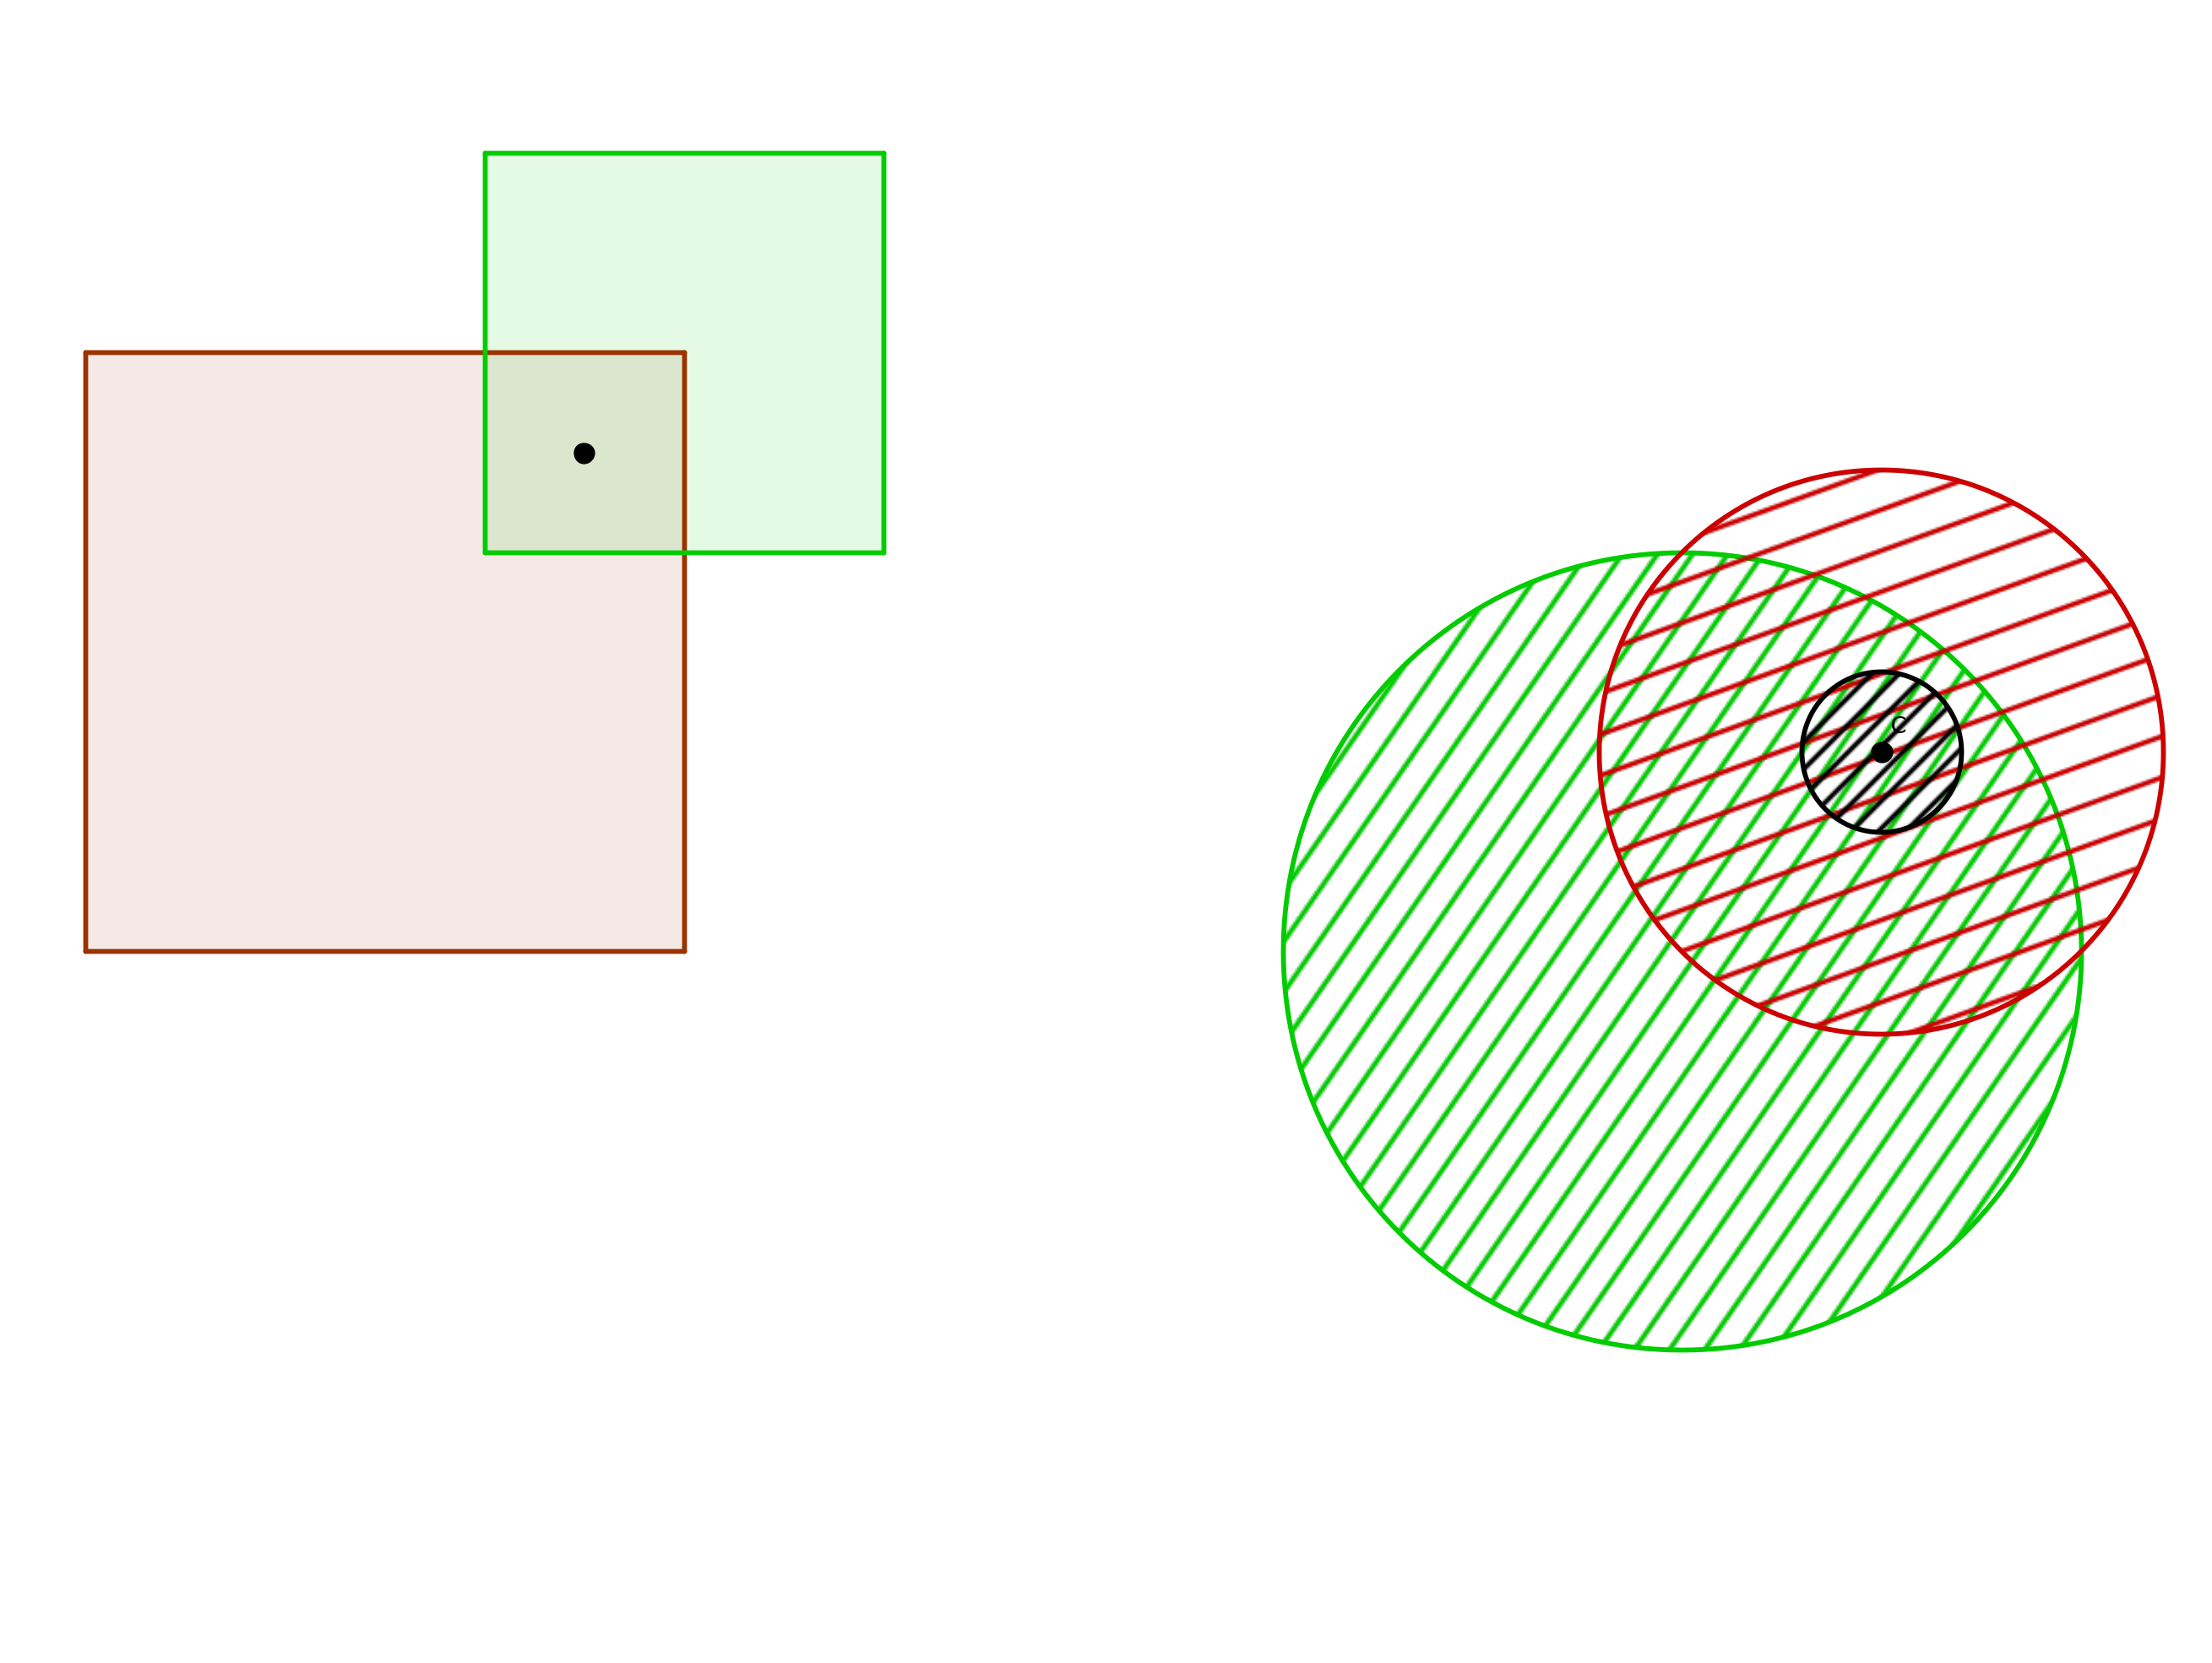
\includegraphics[scale = 0.3]{Figures/Chapter1/basesOfCircularRectangularRegions.png}
    \caption{The basis for $\Bc$ and  $\Bc'$ in  $\R \times \R$  (see example $(2)$).}
    \label{fig_1.2}
\end{figure}

\begin{lemma}\label{1.2.2}
    Let $X$ be a set, and  $\Bc$ be a basis for a topology  $\Tc$ on  $X$. Then 
    $\Tc=\{\bigcup{B}: B \in \Bc\}$.
\end{lemma}
\begin{proof}
    Given a collection $\{B\}$ of basis elements in  $\Bc$, since they are all in  $\Tc$, 
    their unions are also in $\Tc$. Conversely, given  $U \in \Tc$, then for every point 
    $x \in U$, choose a  $B_x \in \B_x$ such that  $x \in B_x \subseteq U$, then  $U=\bigcup_{x \in U}{B_x}$.
\end{proof}

%----------------------------------------------------------------------------------------
%	SECTION 1.3
%----------------------------------------------------------------------------------------

\section{The Order Topology.}

%----------------------------------------------------------------------------------------
%	SECTION 4.3
%----------------------------------------------------------------------------------------

\section{Monotonic Functions and Inverse Functions.}

\begin{definition}
    Let $E \subseteq \R$ be nonempty, and let  $f:E \rightarrow \R$ be a realvalued function. 
    We say that $f$ is \textbf{monotonically increasing} on $E$ if for $x<y$, $f(x) \leq f(y)$. 
    Similarly, $f$ is \textbf{monotonically decreasing} if $f(y) \leq f(x)$. In either case, we call 
    $f$ a \textbf{monotonic} function.
\end{definition}

\begin{example}
    The function $f(x)=x^2$ is not monotonoic on  $I$, but it is monotonically increasing 
    over $[0,\infty)$ and monotonically decreasing over $(-\infty, 0)$. 
\end{example} 

\begin{theorem}\label{4.4.1}
    Suppose that $a, b \in \R$ , with  $a$ and  $b$ distinct, and let  $f$ be contiuous 
    over  $[a,b]$ and differentiable over  $(a,b)$. Then:
        \begin{enumerate}[label=(\arabic*)]
            \item If $f' \geq 0$, for all  $x \in (a,b)$, then $f$ monotonically increasing 
                on $[a,b]$; respectively, if  $f' \leq 0$,  $f$ is monotonically decreasing.

            \item If $f'=0$, for all  $x \in (a,b)$, then $f$ is constant on  $[a,b]$
        \end{enumerate}
\end{theorem}
\begin{proof}
    Assume without loss of generality that $f' \leq 0$, then for any  $a<x_1<x_2<b$, then 
    $f$ is continuous on  $[x_1,x_2]$ and differentiable on $(x_1,x_2)$, hence by the 
    mean value theorem, then there is a $c \in (x_1,x_2)$ such that $f(x_2)f(x_1)=f'(c)(x_2-x_1)$, 
    hence $f(x_2)-f(x_1) \leq 0$, hence $f$ is monotonically decreasing. The case is analogous 
    for  $f'>0$.

    Now suppose that  $f'=0$,  then again by the mean value theorem, there is a  $c \in (x_1,x_2)$ 
    such that $f(x_2)-f(x_1)=f'(c)(x_2-x_1)$, then $f(x_2)-f(x_2)=0$, for $x_1, x_2 \in (a,b)$ 
    arbitrary therefore, $f$ is constant.
\end{proof}

\begin{remark}
    If $f$ and  $g$ are continuous on a nondegenerate inteval,  $[a,b]$, and differentiable 
    on  $(a,b)$, and  $f'=g'$ for all  $x \in (a,b)$, then $f-g$ is constant.
\end{remark}
\begin{proof}
    We repeat the proof for the constant case using the Cauchy mean value theorem; 
    similarly, we can just apply the previous theorem to the function $f-g$.
\end{proof}

Suppose that $f$ is a realvalued function, who has an inverse function  $f^{-1}$. Then 
the graph of  $f^{-1}$ is symmetric to the graph of  $f$ with respect to the line  $y=x$. Then 
visually,  $f^{-1}$ is as smooth as  $f$. Algebraically, we can apply an operation to the graph 
of $f$ to obtain the graph of  $f^{-1}$, and we can observe that smoothness is preserved, however 
we would like to prove this rigorously.

\begin{theorem}\label{4.4.2}
    If $f$ is a  1-1 continuous function of the interval  $I$ onto $\R$, 
    then  $f$ is strictly monotonic on  $I$, and  $f^{-1}$ is continuous and strictly 
    monotonic on $f(I)$.
\end{theorem}
\begin{proof}
    We have that since $f$ is 1-1, then  $f(x)=f(y)$ implies  $x=y$, hence if  $x<y$ 
    are in $I$, then  either $f(x)<f(y)$ or  $f(x)>f(y)$, now if  $f$ is not strictly monotone, then 
    for some $c \in I$, with  $x<c<y$, we have that either  $f(x)$ is inbetween $f(c)$ and  $f(b)$, 
    or  $f(y)$ is between  $f(x)$ and  $f(c)$, hence, by the intermediate value theorem, there is an  $x_1 \in I$ 
    such that $f(x_1)=f(x)$ or $f(x_1)=f(y)$. Then either $x_1=x$ or $x_2=y$ which contradicts the assumption.

    Now suppos that $f$ is strictly increasing on  $I$, since  $f$ is 1-1 ont  $\R$, then 
    $f^{-1}$ exists on  $f(I)$. Now suppose that there are  $y_1,y_2 \in f(I)$ such that 
    $ y_1<y_2$ but $f^{-1}(y_1) \geq f^{-1}(y_2)$, and since $f$ is increasing, then  $f(x_1) \geq f(x_2)$, which 
    is absurd. We also have that $f(I)$ is an interval for if  $I=[a,b]$, then  $f([a,b])=[f(a)f(b)]$ by 
    the intermediate value theorem.

    Now fix  $y_0 \in f(I)$, and let $\epsilon>0$, since $f^{-1}$ is strictly increasing, on $f(I)$ by 
    the above assumption, if $y_0$ is not a right endpoint of $f(I)$, then  $f^{-1}(y_0)$ is not 
    a  right endpoint of  $I$, then  there is an $0<\epsilon_0<\epsilon$ with $\epsilon+\epsilon_0 \in I$. Let  $\delta=f(x_0+\epsilon_0)-f(x_0)$, 
    and suppose that $0<y-y_0<\delta$, then $y_0<y<y_0+\delta=f(x_0+\epsilon_0)$, then since $f^{-1}$ is strictly 
    increasing, it follows that  $x_0<x<x+\epsilon_0$, hence we have that $0<f^{-1}(y)-f^{-1}(y_0)<\epsilon$, 
    that is $f^{-1}(y_0+)$ exists, similatly, if $y_0$ is not a left endpoint of $I$, then  $f^{-1}(y_0-)$ 
    exists. In both cases, we have that $f^{-1}(y_0\pm)=f(y_0)$. Therefore, $f^{-1}$ is contiuous.
\end{proof}

\begin{theorem}[The Inverse Function Theorem]\label{4.4.3}
    Let $f$ be a 1-1 continuous function of an open interval  $I$ onto  $\R$. If  $a \in f(I)$, 
    and if  $f'(f^{-1}(a)) \neq 0$ exists, then  $f^{-1}$ is differentiable at $a$, and 
        \begin{equation}
            (f^{-1})'=\frac{1}{f'}
        \end{equation} 
\end{theorem}
\begin{proof}
    We have that $f(f(^{-1})(x))=x$, if $f$ and $f^{-1}$ are both differentiable, then 
    the chain rule yields the appropriate result. It remains to show that  $f^{-1}$ is 
    differentiable.

    By the previous theorem, we have that  $f$ is strictly monotonic, and say, without 
    loss of generalilty, that  $f$ is strictly increasing. Then  $f^{-1}$ exists, is continuous, and 
    is strictly increasing on $f(I)$. Let  $x_0=f^{-1}(a)$, then there are $c,d \in I$ such that 
    $x_0 \in (c,d) \subseteq I$, thus by the intermediate value theorem, we have that  $f((c,d))=(f(c),f(d))$ which 
    contains  $f(x_0)=a$. Then for $h \neq 0$ sufficiently small  $a+h \in (f(c),f(d))$, 
    hence $f^{-1}(a+h)$ is well defined. Now let  $x=f^{-1}(a+h)$, then  $f(x)=a+h=f(x_0)+h$, 
    thus $h=f(x)-f(x_0)$. Since $f$ is continuous, we have that as  $x \rightarrow x_0$, $h \rightarrow 0$, 
    hence  $x-x_0=f^{-1}(a+h)-f^{-1}(a) \rightarrow 0$, hence $\frac{f^{-1}(a+h)-f^{-1}(a)}{h}=
    \frac{x-x_0}{f(x)-f(x_0)}$ which exists by the continuity of $f$, thus  $f^{-1}$ is differentiable at  $a$.
\end{proof}

\begin{example}
    Take $f(x)=1$ for  $x \in \Q$ and  $f(x)=0$ for  $x \in \com{\R}{\Q}$, which is not 
    continuous at any $x$, also notice that  $x$ is not monotonic.
\end{example}

\begin{lemma}\label{4.4.4}
    Suppose that $f$ is monotonic on  $[a,b]$, if  $x_0 \in [a,b)$, then $f(x_0+)$ exists and 
    $f(x_0) \leq f(x_0+)$ or $f(x_0) \geq f(x_0+)$ (if it is increasing or decreasing respectively). Moreover, 
    if $x_0 \in (a,b]$, then $f(x_0-)$ exists and $f(x_0-) \leq f(x_0)$ or $f(x_0-) \geq f(x_0)$.
\end{lemma}
\begin{proof}
    Fix $x_0 \in [a,b]$, by the symmetry, it suffices to show that $f(x_0-)$ exists and that 
    $f(x_0-) \leq f(x_0)$ if $f$ is increasing. Set  $E=\{f(x):a<x<x_0\}$ and let $s=\sup{E}$. We have 
    $f (x_0)$ is an upeprbound, thus $s$ is finite, and  $s \leq f(x_0)$. It remains to show that $s=f(x_0-)$.

    Now given $\epsilon>0$, by the approximation property, there is an $x_1 \in (a,x_0)$ such that 
    $s-\epsilon<f(x) \leq s$. Since  $f$ is increasing, then we have  $s-\epsilon<f(x_1)<f(x) \leq s$, so 
    choose $\delta=x_0-x_1>0$, then for $-\delta<x-x_0<0$, we have that $|f(x)-s|<\epsilon$, and we are 
    done.
\end{proof}

\begin{theorem}\label{4.4.5}
    If $f$ is monotonic on an interval  $I$, then  $f$ has at most countably many discontinuities on  $I$.
\end{theorem}
\begin{proof}
    Suppose that $f$ is monotonically increasing, without loss of generality. We know that the 
    countable union of atmost countable sets is countable. It suffices to show that the set 
    of all discontinuities of  $f$ is a coutnable union of atmost countable sets.

    Notice that  $\R=\bigcup_{n=1}^{\infty}{[-n,n]}$, now let  $I$ be a closed, bounded, interval  $[a,b]$, 
    and let $E$ be the set of all discontinuities of  $f$ on  $(a,b)$. By lemma \ref{4.4.4}, we have that 
    $f(x-) \leq f(x) \leq f(x+)$, then we see that  $f$ is discontinuous at  $x$ if and only if  $0<f(x+)-f(x-)$. 
    Let  $A_j=\{x \in I: f(x+)-f(x-) \geq \frac{1}{j}\}$, then $A_j \subseteq E$, and we have 
    $E=\bigcup_{j=1}^{\infty}{A_j}$. We would like to show that  $A_j$ is finite for all  $j$.

    For suppose not, then there is a  $j_0$ such that $A_{j_0}$ is infinite, then pick $a \leq x_1<x_2<\dots 
    \leq b\in A_{j_0}$, with $f(x_k+)-f(x_k-)>\frac{1}{j_0}$ for all $k$. Then $f(b)-f(a) \geq f(b)-f(x_1-) 
    \geq f(x_1+)-f(x_1-)>\frac{1}{j_0} \geq f(x_2+)-f(x_1-)=f(x_2+)-f(x_2-)+f(x_2-)-f(x_1-)>\frac{1}{j_0}$, 
    continuing along this line, we get that $f(b)-f(a) \geq \frac{n}{j_0}$ for all $n \geq 1$, which 
    implies that  $f(b)-f(a)$ is infinite, which is a contradiction. Thus  $A_j$ must be finite.
\end{proof}

\begin{figure}
    \centering
    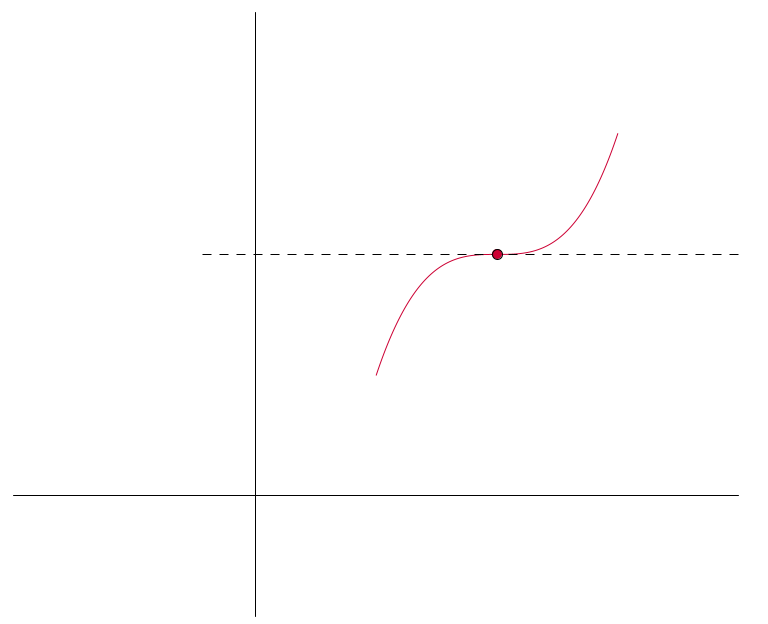
\includegraphics[scale = 0.3]{figures/meanValueDeriv.png}
    \caption{The intermediate value theorem for derviavtives.}
    \label{fig_4.2}
\end{figure}

\begin{theorem}[The Intermediate Value Theorem for Derivatives]\label{4.4.5}
    Suppose that $f$ is differentiable on a closed interval  $[a,b]$, where  $f'(a) \neq g('b)$. If  $y_0 \in \R$ such that $f'(a)<y_0<f'(b)$, then there is an $x_0 \in (a,b)$ such that $f'(x_0)=y_0$.
\end{theorem}
\begin{proof}
    Suppose that $f'(a)<y_0<f'(b)$, now suppose without loss of generality that $f'(a)<f'(b)$. Now let $F(x)=f(x)-y_0x$, for $x \in [a,b]$. We have that $F$ is differentiable on  $(a,b)$, then by the extreme value theorem, $F$ has a local maximum, and a local minumum, let  $F(x_0)$ is a local minimum on $[a,b]$. We have that  $F'(a)=f'(a)-y_0<0$, which is decreasing, so for $h$ sufficiently small, we have  $F(a+h)-F(a)<0$, hence  $F(a)$ cannot be the minumum, hence  $x_0 \neq a$. Similarly,
    $F'(b)=f'(b)-y_0>0$, which is increasing, by similar reasoning, we have that $F(b+h)-F(b)>0$ for  $h$ sufficiently small, hence $F(b)$ cannot be a local maximum, so  $x_0 \neq b$. Thus $x_0 \in (a,b)$. Now since $F(x_0)$ is a local minumum, then we have that $F'(x_0)=0$, hence $f'(x_0)=y_0$
\end{proof}
\begin{remark}
    If in the proof we assume that $f'(a)>y_0>f'(b)$, then we consider $F(x_0)$ to be a local maximum.
\end{remark}

%----------------------------------------------------------------------------------------
%	SECTION 1.1
%----------------------------------------------------------------------------------------

\section{Special Sequences}

\begin{theorem}\label{3.5.1}
    Let $n, p \in \Z^+$. Then the following hold as  $n \rightarrow \infty$.
        \begin{enumerate}[label=(\arabic*)]
            \item $\lim{\frac{1}{n^p}}=0$.

            \item $\lim{\sqrt[p]{n}}=1$.

            \item $\lim{\sqrt[n]{n}}=1$.

            \item If $\alpha \in \R$, then  $\lim{\frac{n^{\alpha}}{(1+p)^n}}=0$.

            \item If $|x|<1$, then  $\lim{x^n}=0$.
        \end{enumerate}
\end{theorem}
\begin{proof}
   \begin{enumerate}[label=(\arabic*)]
       \item Let $n>\sqry[p]{\frac{1}{\epsilon}}$; then $|\frac{1}{n^p}|<\epsilon$.

       \item If $p=1$, we are done. If  $p>1$, let  $x_n=\sqrt[n]{p}-1$, then  $x_n>0$. 
           By the binomial theorem, $1+nx_n \leq (1+x_n)^p=p$, hence $0 \leq x_n \leq \frac{p-1}{p}$. 
           Now if $1>p>0$, then  $ \frac{1}{p}>0$, so we notice that $0 \leq \frac{1}{x_n} \leq \frac{1}{\frac{p-1}{n}}$.

       \item Let $x_n=\sqrt[n]{n}-1$, then  $x_n \geq 0$, then by the binomial theorem again, 
           $n=(1+x_n)^n \geq \frac{n(n-1)}{2}x_n^2$, then $0 \leq x_n \leq \sqrt{\frac{2}{n-1}}$.

       \item Let $k \in \Z^+$ such that  $k>\alpha$. Then  $n>2k$,let  $(1+p)^n> {n \choose k}p^k>
           \frac{n^kp^k}{2^kk!}$. So $0<\frac{n^{\alpha}}{(1+p)^n}<\frac{2^kk!}{p^k}n^{\alha-k}$, since 
           $\alpha-k<0$,  $n^{\alpha-k} \rightarrow 0$ and we are done.

       \item Take  $\alpha=0$, and let  $x=\frac{1}{1+p}$, then the result follow.
   \end{enumerate} 		
\end{proof}

%----------------------------------------------------------------------------------------
%	SECTION 1.1
%----------------------------------------------------------------------------------------

\section{Monotonic Functions.}

\begin{definition}
    Let $f$ be a realvalued function on an interval  $(a,b)$. We say that  $f$ is 
    \textbf{monotonically increasing} on $(a,b)$ if  $a<x<y<b$ implies  $f(x) \leq f(y)$. 
    We say that  $f$ is \textbf{monotonically decreasing} on $(a,b)$ if  $a<x<y<b$ 
    implies  $f(y) \leq f(x)$. We say $f$ is \textbf{monotonic} if it is either monotonically 
    increasing or monotonically decreasing.
\end{definition}

\begin{theorem}\label{5.6.1}
    Let $f$ be monotonic on $(a,b)$ then $f(x+)$ and  $f(x-)$ exist at every point of 
    $(a,b)$ and $\sup{f}=f(x-)$ and  $\inf{f}=f(x+)$, and the following hold:
        \begin{enumerate}[label=(\arabic*)]
            \begin{enumerate}[label=(\arabic*)]
                \item If $f$ is monotonically increasing $f(x-) \leq f(x) \leq f(x+)$

                \item If $f$ is monotonically decreasing $f(x+) \leq f(x) \leq f(x-)$
            \end{enumerate}		
        \end{enumerate}
\end{theorem}
\begin{proof}
    We prove only $(1)$, since  $(2)$ is analogous. Suppose that $f$ is monotonically 
    increasing, clearly,  $f$ has an upperbound  $A$ for which  $A \leq f$. Now let  $\epsilon>0$, 
    then there is a  $\delta>0$ for which  $a<x-\delta<x$, and  $A-\epsilon<f(x-\delta) \leq A$.  Then we have 
    $f(x-\delta)<f(t) \leq A$ for all  $x-\delta<t<x$, then we get  $|f(t)-A|<\epsilon$, hence 
    $f(x-)=A$, Similarly, we get  $f(+)-\inf{f}$. Now since  $\sup{f} \leq f \leq inf{f}$, 
    we get the desired result.
\end{proof}

\begin{corollary}
    Monotonic functions have no infinite discontinuities.		
\end{corollary}

\begin{theorem}\label{5.6.2}
    Let $f$ be monotonic on  $(a,b)$, then the set of all  points of $(a,b)$ for which 
    $f$ is  discontinuous is atmost countable.
\end{theorem}
\begin{proof}
    Suppose, without loss of generality that $g$ is monotonically increasing, and let  $E$ 
    be the set of all points of  $(a,b)$ for which  $f$ is discontinuous. By the density of 
    $\Q$ in  $\R$, for each $x \in E$ associate $r(x) \in \Q$ such that $f(x+)<f(x)<f(x-)$. 
    Since  $x_1 < x_2$ implies $f(x_1+) \leq f(x_2-)$, then $r(x_1) \neq r(x_2)$, thus 
    $x_1 \neq x_2$, and so $r$ is a 1-1 mapping of  $E$ into  $\Q$.
\end{proof}

Now, given a countable $E$ in an interval  $(a,b)$, we can construct a monotonic function $f$ that 
is discontinuous at every point in  $E$ and continuous everywhere else. Arrange  the points of  
$E$ into a sequence  $\{x_n\}$ and let  $\{c_n\}$ be a sequence such that  $c_n>0$ for 
all  $n \in \Z^+$, such that  $\sum{c_n}$ converges. Define  $f(x)=\sum_{x_n<x}{c_n}$, for 
$x \in (a,b)$. Then we have that 
    \begin{enumerate}[label=(\arabic*)]
        \item $f$ is monotonically increasing on $(a,b)$.
            
        \item $f$ is discontinuous at every point in $E$ with $f(x_n+)-f(x_n-)=c_n$.

        \item $f$ is continuous at every point in $\com{(a,b)}{E}$.
    \end{enumerate}

\begin{definition}
    Let $f$ be a realvalued function defined on an interval $(a,b)$. We say that $f$ is 
    \textbf{continuous form the right} if $f(x+)=f(x)$, and we say $f$ is \textbf{continuous from the 
    left} if $f(x-)=f(x)$.
\end{definition}

                         % If you want add this chapter remove the comment (%).
%\input{chapters/Conclusion.tex}    				   % This is the last Chapter

%\appendix									           % End of the body of the thesis, begin of the appendices.
%\makeappendicespage		                           % Create a page with "APPENDICES" in the middle.

%% Appendix
%==========================================================================
\chapter{}
\label{AppA}
			           % This is the appendix A.
%% Appendix
%==========================================================================
\chapter{TITLE OF APPENDIX B}
\label{AppB}


Appendix B goes here.			           % This is the appendix B. For more appendices: \input{AppendixC.tex}
%%       Make List of References
%%%%%%%%%%%%%%%%%%%%%%%%%%%%%%%%%%%%%%%%%%%%%%%%%%%%%%%%%%%%%%%%
%% Note: I use BibTeX, but have coded in thebibliography environment
%%       to use for this example only.
%%%%%%%%%%%%%%%%%%%%%%%%%%%%%%%%%%%%%%%%%%%%%%%%%%%%%%%%%%%%%%%%


									% unstr is the same as
\begin{thebibliography}{1}
\bibliographystyle{plain}


\bibitem{sperber} A. Adolphson and S. Sperber. 
\newblock $p$-adic Estimates for Exponential Sums and the of Chevalley-Warning.
\newblock {\it Ann. Sci. Ec. Norm. Super.}, $4^{e}$ s\'erie,  {\bf 20}, 545--556, 1987.

\bibitem{acgmr} R. A. Arce-Nazario, F. N. Castro, O. E. Gonz\'alez, L. A. Medina and I. M. Rubio.
\newblock New families of balanced symmetric functions and a generalization of Cuscik, Li and P. St$\check{\mbox{a}}$nic$\check{\mbox{a}}$.
\newblock {\it Designs, Codes and Cryptography} {\bf 86}, 693--701, 2018.

\bibitem{ax} J. Ax.
\newblock Zeros of polynomials over finite fields. 
\newblock {\it Amer. J. Math.}, {\bf 86}, 255--261, 1964.

\bibitem{BCP} M. L. Bileschi, T.W. Cusick and D. Padgett.
\newblock Weights of Boolean cubic monomial rotation symmetric functions.
\newblock {\it Cryptogr. Commun.}, {\bf 4}, 105--130, 2012.

\bibitem{browncusick} A. Brown and T. W. Cusick.
\newblock Recursive weights for some Boolean functions. 
\newblock  {\it J. Math. Cryptology}, {\bf 6(2)}, 105--135, 2012.

\bibitem{cai} J. Cai, F. Green and T. Thierauf. 
\newblock On the correlation of symmetric functions.
\newblock {\it Math. Systems Theory}, {\bf 29}, 245--258, 1996.

\bibitem{canteaut} A. Canteaut and M. Videau.
\newblock Symmetric Boolean Functions.
\newblock {\it IEEE Trans. Inf. Theory} {\bf 51(8)}, 2791--2881, 2005.

\bibitem{Davis}
\newblock Philip Davis. Circulant Matrices.
\newblock Chelsea publishing, Second Edition,1994.

\bibitem{cgm3} F. N. Castro, O. E. Gonz\'alez and L. A. Medina.
\newblock Diophantine Equations With Binomial Coefficients and Perturbations of Symmetric Boolean Functions.
\newblock {\it IEEE Trans. Inf. Theory}, {\bf 64(2)}, 1347--1360, 2018.

\bibitem{cm1} F. N. Castro and L. A. Medina. 
\newblock Linear Recurrences and Asymptotic Behavior of Exponential Sums of Symmetric Boolean Functions. 
\newblock {\it Elec. J. Combinatorics}, 18:\#P8, 2011.

\bibitem{cm2} F. N. Castro and L. A. Medina. 
\newblock Asymptotic Behavior of Perturbations of Symmetric Functions.  
\newblock {\it Annals of Combinatorics}, 18:397--417, 2014.

\bibitem{cm3} F. N. Castro and L. A. Medina. 
\newblock Modular periodicity of exponential sums of symmetric Boolean functions.
\newblock {\it Discrete Appl. Math.} {\bf 217}, 455--473, 2017.

\bibitem{cms} F. N. Castro, L. A. Medina and P. St$\check{\mbox{a}}$nic$\check{\mbox{a}}$.
\newblock Generalized Walsh transforms of symmetric and rotation symmetric Boolean functions are linear recurrent.
\newblock {\it Appl. Algebra Eng. Commun. Comput.}, DOI 10.1007/s00200-018-0351-5, 2018.

\bibitem{ccms} F. N. Castro, R. Chapman, L. A. Medina, and L. B. Sep\'ulveda.  
\newblock Recursions associated to trapezoid, symmetric and rotation symmetric functions over Galois fields.
\newblock {\it Discrete Mathematics.},{\bf 341}, 1915--1931, 2018.

\bibitem{cusick4} T. W. Cusick. 
\newblock Hamming weights of symmetric Boolean functions.
\newblock {\it Discrete Appl. Math.} {\bf 215}, 14--19, 2016.

\bibitem{cusickArXiv} T. W. Cusick.
\newblock Weight recursions for any rotation symmetric Boolean functions.
\newblock {\it IEEE Trans. Inf. Theory}, {\bf 64}, 2962 - 2968, 2018.

\bibitem{cusickjohns} T. W. Cusick and B. Johns.
\newblock Recursion orders for weights of Boolean cubic rotation symmetric functions.
\newblock {\it Discr. Appl. Math.}, {\bf 186}, 1--6, 2015.

\bibitem{cusick2} T. W. Cusick, Y. Li, and  P. St$\check{\mbox{a}}$nic$\check{\mbox{a}}$.
\newblock Balanced Symmetric Functions over $GF(p)$.
\newblock {\it IEEE Trans. Inf. Theory}, {\bf 5}, 1304--1307, 2008.

\bibitem{cusickstanica} T.W. Cusick and P. St$\check{\mbox{a}}$nic$\check{\mbox{a}}$.
\newblock Fast evaluation, weights and nonlinearity of rotation symmetric functions.
\newblock {\it Discr. Math.}, {\bf 258}, 289--301, 2002.

\bibitem{dalaimaitrasarkar} D. K. Dalai, S. Maitra and S. Sarkar. 
\newblock Results on rotation symmetric Bent functions.
\newblock {\it Second International Workshop on Boolean Functions: Cryptography and
Applications, BFCA'06}, publications of the universities of Rouen and Havre, 137--156, 2006.

\bibitem{fengliu} K. Feng and F. Liu. 
\newblock New Results On The Nonexistence of Generalized Bent Functions. 
\newblock {\it IEEE Trans. Inf. Theory} {\bf 49},  3066--3071, 2003.

\bibitem{ggz} Y. Guo, G. Gao, Y. Zhao.
\newblock Recent Results on Balanced Symmetric Boolean Functions.
\newblock {\it IEEE Trans. Inf. Theory} {\bf 62 (9)}, 5199--5203, 2016.

\bibitem{hell} M. Hell, A. Maximov and S. Maitra. 
\newblock On efficient implementation of search strategy for rotation symmetric Boolean functions. 
\newblock {\it Ninth International Workshop on Algebraic and Combinatorial Coding Theory, ACCT 2004}, Black Sea Coast, Bulgaria,
2004.

\bibitem{hg} Y. Hu and G. Xiao.
\newblock Resilient Functions Over Finite Fields.
\newblock {\it IEEE Trans. Inf. Theory} {\bf 49},  2040--2046, 2003.

\bibitem{ims} E. J. Iona\c{s}cu, Thor Martinsen, Pantelimon St$\check{\mbox{a}}$nic$\check{\mbox{a}}$.
\newblock Bisecting binomial coefficients.
\newblock {\it Discrete Appl. Math.} {\bf 227} (2017) 70--83.

\bibitem{fspectrum} M. Kolountzakis, R. J. Lipton, E. Markakis, A. Metha and N. K. Vishnoi. 
\newblock On the Fourier Spectrum of Symmetric Boolean Functions.
\newblock {\it Combinatorica}, {\bf  29}, 363--387, 2009.

\bibitem{KScW} P.V. Kumar, R.A. Scholtz, and L.R. Welch. 
\newblock Generalized Bent Functions and Their Properties.
\newblock {\it J. Combinatorial Theory (A)}, {\bf 40}, 90--107, 1985.

\bibitem {licusick1} Y. Li and T.W. Cusick. 
\newblock Linear Structures of Symmetric Functions over Finite Fields.
\newblock {Inf. Processing Letters} {\bf 97}, 124--127, 2006.

\bibitem{licusick2} Y. Li and T. W. Cusick. 
\newblock Strict Avalanche Criterion Over Finite Fields.
\newblock {\it J. Math. Cryptology}  {\bf 1(1)}, 65--78, 2006.

\bibitem{llm}M. Liu, P. Lu and G.L. Mullen. 
\newblock Correlation-Immune Functions over Finite Fields.
\newblock {\it IEEE Trans. Inf. Theory} {\bf 44}, 1273--1276, 1998.

\bibitem{maxhellmaitra} A. Maximov, M. Hell and S. Maitra. 
\newblock Plateaued Rotation Symmetric Boolean Functions on Odd Number of Variables. 
\newblock {\it First Workshop on Boolean Functions:Cryptography and Applications, BFCA'05}, publications of the universities of Rouen and Havre, 83--104, 2005.

\bibitem{mitchell}  C. Mitchell.
\newblock Enumerating Boolean functions of cryptographic significance.
\newblock {\em J. Cryptology} {\bf 2} (3), 155--170, 1990.

\bibitem{mm1} O. Moreno and C. J. Moreno.
\newblock Improvement of the Chevalley-Warning and the Ax-Katz theorems.
\newblock {\it Amer. J. Math.}, {\bf 117}, 241--244, 1995.

\bibitem{mm} O. Moreno and C. J. Moreno.
\newblock The MacWilliams-Sloane Conjecture on the Tightness of the Carlitz-Uchiyama Bound and the Weights of Dual of BCH Codes.
\newblock {\it IEEE Trans. Inform. Theory}, {\bf 40},  1894--1907, 1994.

\bibitem{parkerpott} M. G. Parker and A. Pott. 
\newblock On Boolean functions which are bent and negabent.
\newblock {\it Proc. Int. Conf. Sequences, Subsequences, Consequences},
LNCS-4893, 9--23, 2007.

\bibitem{piequ} J. Pieprzyk and C.X. Qu.
\newblock Fast hashing and rotation-symmetric functions.
\newblock {\it J. Universal Comput. Sci.}, {\bf 5 (1)}, 20--31, 1999.

\bibitem{rp} C. Riera and M. G. Parker.
\newblock Generalized bent criteria for Boolean functions.
\newblock {\it IEEE Trans. Inform. Theory} {\bf 52} (9), 4142--4159, 2006.

\bibitem{fdegree} A. Shpilka and A. Tal.
\newblock On the Minimal Fourier Degree of Symmetric Boolean Functions.
\newblock {\it Combinatorica}, {\bf 88}, 359--377, 2014.

\bibitem{stanicamaitra} P. St$\check{\mbox{a}}$nic$\check{\mbox{a}}$ and S. Maitra. 
\newblock Rotation Symmetric Boolean Functions -- Count and Cryptographic Properties. 
\newblock {\it Discr. Appl. Math.}, {\bf 156}, 1567--1580, 2008

\bibitem{stanicamaitraclark} P. St$\check{\mbox{a}}$nic$\check{\mbox{a}}$, S. Maitra and J. Clark. 
\newblock Results on Rotation Symmetric Bent and Correlation Immune Boolean Functions. 
\newblock {\it Fast Software Encryption, FSE 2004}, Lecture Notes in Computer Science, {\bf 3017}, 161--177. SpringerVerlag, 2004.

\end{thebibliography}

\addcontentsline{toc}{extrachapter}{BIBLIOGRAPHY}%







%\bibliography{referencefiles/references.bib} 		% Use the References.bib file

%\backmatter %

%\biography{										% Add the Biography pages if you want.
%% Biography.tex

Here goes the Biography.

Use the file: \fn{Biography.tex}

%%%% CESAR ACEROS %%%% Biography %%%%%

%Cesar A Aceros was born in Dec, 23 of 1970 in Bucaramanga, Santander, Colombia. Cesar is son of Rodolfo Aceros Fajardo and Esperanza Moreno de Aceros. In October of 1995 receive the Electronic Engineer degree from the Pontificia Universidad Javeriana. He works in Conalvidrios S.A. the second in importance bottle glass factory in Colombia and later in August of 1996, he works at the Universidad Pontificia Bolivariana in Bucaramanga as a proffesor. In 2003 he left Colombia and start the M.S. studies at the University of Puerto Rico at Mayag\"uez. 


%%%% ALBERTO SANTANA %%%% Biography %%%%%

%was born on May 2$^{\rm nd}$, 1972, in San Germ\'an, Puerto Rico. Alberto is the son of Radam\'es Santana and N\'elida Vargas. In June 1995 he received his B.S.\ degree in chemistry from the University of Puerto Rico, Mayag\"uez Campus. In August of the same year, he started his graduate education. He worked under the supervision of Dr.\ Samuel P.\ Hern\'andez. Alberto spent more than two years doing research in the area of surface enhanced Raman spectroscopy (SERS). In June of 1998, Alberto received his second academic degree, a M.S.\ in chemistry from the same university.
%
%After doing experimental work, Alberto decided to continue his academic formation, but this time it would be in another area of chemistry. He came to the USA in January of 1998 and joined the Physical Chemistry Division of the Chemistry Department at the University of Florida. After completing his written and oral examinations, Alberto was admitted to the Ph.D.\ program and started his research on the theoretical and computational aspects of quantum molecular dynamics applied to surface chemistry under the supervision of Dr. David A. Micha. 
			
%}

%%%%%%%%%%%%%%%%%%%%%%%%%%%%%%%%%%%%%%%%%%%%%%%
%%  Create a General Audience Abstract      %%%
%%%%%%%%%%%%%%%%%%%%%%%%%%%%%%%%%%%%%%%%%%%%%%%

%\begin{simpleenv}{}{}{}{}%
%\pagestyle{empty}
%\begin{flushleft}
%\Title\\*[\BaseDiff\baselineskip]
%\FullName\\%
%(787) XXX-XXXX\\%
%Department of \Department \\%
%Chair: \Chair\\%
%Degree: \DegreeType\\%
%Graduation Date: \GradMonth~\GradYear%
%\end{flushleft}
%\GoDouble%
%% GeneralAudienceAbstract.tex


This is the general Audience Abstract.

Use the file: \fn{GeneralAudienceAbstract.tex}

%Density matrix theory is applied to the CO/Cu(001)
%adsorbate/substrate system to evaluate the nonlinear photodesorption yield of CO versus pulse fluence through model calculations. The dynamics of molecular photodesorption from a metal surface is described by the nonlinear optical response resulting from the interaction of a femtosecond pulsed laser with a metal surface. Our formalism uses the Liouville-von Neumann equation, with an effective hamiltonian which includes the effects of energy dissipation into the metal. The nonlinear response of the substrate to femtosecond excitation is taken into account by solving modified optical Bloch equations with relaxation terms to account for the effects of energy dissipation. Our previous density matrix treatment has been extended to include several quantum states, and to treat rotational motions of the desorbing molecule. Results for intense lasers including chirping at pulse wavelengths around 620 nm have also been obtained.

%\end{simpleenv}

					                   % This file create the Bibliography, Biography and general abstrac for the thesis.
\end{document} 